\documentclass[fontsize=12pt, paper=a4, headinclude, twoside=true, parskip=half+, pagesize=auto, numbers=noenddot, plainheadsepline, open=right, toc=listof, toc=bibliography]{scrreprt}
% PDF-Kompression
\pdfminorversion=5
\pdfobjcompresslevel=1
% Allgemeines\\
\raggedbottom
\usepackage{blindtext}
\usepackage{caption}
\usepackage[automark]{scrpage2} % Kopf- und Fußzeilen
\usepackage{amsmath,marvosym} % Mathesachen
\usepackage[T1]{fontenc} % Ligaturen, richtige Umlaute im PDF
\usepackage[utf8]{inputenc}% UTF8-Kodierung für Umlaute usw
% Schriften
\usepackage{textcomp}
\usepackage{mathpazo} % Palatino für Mathemodus
%\usepackage{mathpazo,tgpagella} % auch sehr schöne Schriften
\usepackage{setspace} % Zeilenabstand
\onehalfspacing % 1,5 Zeilen
% Schriften-Größen
\setkomafont{chapter}{\Huge\rmfamily} % Überschrift der Ebene
\setkomafont{section}{\Large\rmfamily}
\setkomafont{subsection}{\large\rmfamily}
\setkomafont{subsubsection}{\large\rmfamily}
\setkomafont{chapterentry}{\large\rmfamily} % Überschrift der Ebene in Inhaltsverzeichnis
\setkomafont{descriptionlabel}{\bfseries\rmfamily} % für description Umgebungen
\setkomafont{captionlabel}{\small\bfseries}
\setkomafont{caption}{\small}
\usepackage{titlesec}
\titlespacing{\section}{0pt}{\parskip}{-0.1\baselineskip}
\titlespacing{\subsection}{0pt}{\parskip}{-0.3\baselineskip}
\titlespacing{\subsubsection}{0pt}{\parskip}{-0.5\baselineskip}

% Sprache: Deutsch
\usepackage[ngerman]{babel} % Silbentrennung
% PDF
\usepackage[ngerman,pdfauthor={Martin Bretschneider},  pdfauthor={Martin Bretschneider}, pdftitle={Vorlage für LaTeX}, breaklinks=true,baseurl={http://www.bretschneidernet.de/tips/thesislatex.html}]{hyperref}
\usepackage[final]{microtype} % mikrotypographische Optimierungen
\usepackage{url}
\usepackage{pdflscape} % einzelne Seiten drehen können
% Tabellen
\usepackage{multirow} % Tabellen-Zellen über mehrere Zeilen
\usepackage{multicol} % mehre Spalten auf eine Seite
\usepackage[multiple]{footmisc} %mehrere Fusszeilen
\usepackage{tabularx} % Für Tabellen mit vorgegeben Größen
\usepackage{longtable} % Tabellen über mehrere Seiten
\usepackage{array}
%  Bibliographie
\usepackage{bibgerm} % Umlaute in BibTeX
% Tabellen
\usepackage{multirow} % Tabellen-Zellen über mehrere Zeilen
\usepackage{multicol} % mehre Spalten auf eine Seite
\usepackage{tabularx} % Für Tabellen mit vorgegeben Größen
\usepackage{array}
\usepackage{float}
% Bilder
\usepackage{graphicx} % Bilder
\usepackage{wrapfig}
\usepackage{color} % Farben
\graphicspath{{images/}}
\DeclareGraphicsExtensions{.pdf,.png,.jpg} % bevorzuge pdf-Dateien
\usepackage{subfigure} % mehrere Abbildungen nebeneinander/übereinander
\newcommand{\subfigureautorefname}{\figurename} % um \autoref auch für subfigures benutzen
\usepackage[all]{hypcap} % Beim Klicken auf Links zum Bild und nicht zu Caption gehen
% Bildunterschrift
\setcapindent{0em} % kein Einrücken der Caption von Figures und Tabellen
\setcapwidth[c]{0.9\textwidth}
\setlength{\abovecaptionskip}{0.2cm} % Abstand der zwischen Bild- und Bildunterschrift
% Quellcode
\usepackage{listings} % für Formatierung in Quelltexten
\usepackage{chngcntr}
\counterwithout{footnote}{chapter}
\definecolor{grau}{gray}{0.25}
\lstset{
	extendedchars=true,
	basicstyle=\small\ttfamily,
	%basicstyle=\footnotesize\ttfamily,
	tabsize=2,
	keywordstyle=\textbf,
	commentstyle=\color{grau},
	stringstyle=\textit,
	numbers=left,
	numberstyle=\tiny,
	% für schönen Zeilenumbruch
	breakautoindent  = true,
	breakindent      = 2em,
	breaklines       = true,
	postbreak        = ,
	prebreak         = \raisebox{-.8ex}[0ex][0ex]{\Righttorque},
}
% linksbündige Fußboten
\deffootnote{1.5em}{1em}{\makebox[1.5em][l]{\thefootnotemark}}

\typearea{14} % typearea berechnet einen sinnvollen Satzspiegel (das heißt die Seitenränder) siehe auch http://www.ctan.org/pkg/typearea. Diese Berechnung befindet sich am Schluss, damit die Einstellungen oben berücksichtigt werden
% für autoref von Gleichungen in itemize-Umgebungen
\makeatletter
\newcommand{\saved@equation}{}
\let\saved@equation\equation
\def\equation{\@hyper@itemfalse\saved@equation}
\makeatother 


% Eigene Befehle %%%%%%%%%%%%%%%%%%%%%%%%%%%%%%%%%%%%%%%%%%%%%%%%%5
% Matrix
\newcommand{\mat}[1]{
      {\textbf{#1}}
}
\newcommand{\todo}[1]{
      {\colorbox{red}{ TODO: #1 }}
}
\newcommand{\todotext}[1]{
      {\color{red} TODO: #1} \normalfont
}
\newcommand{\info}[1]{
      {\colorbox{blue}{ (INFO: #1)}}
}
% Hinweis auf Programme in Datei
\newcommand{\datei}[1]{
      {\ttfamily{#1}}
}
\newcommand{\code}[1]{
      {\ttfamily{#1}}
}
% bild mit defnierter Breite einfügen
\newcommand{\bild}[4]{
  \begin{figure}[!hbt]
    \centering
      \vspace{1ex}
      \includegraphics[width=#2]{images/#1}
      \caption[#4]{\label{img.#1} #3}
    \vspace{1ex}
  \end{figure}
}
% bild mit eigener Breite
\newcommand{\bilda}[3]{
  \begin{figure}[!hbt]
    \centering
      \vspace{1ex}
      \includegraphics{images/#1}
      \caption[#3]{\label{img.#1} #2}
      \vspace{1ex}
  \end{figure}
}


% Bild todo
\newcommand{\bildt}[2]{
  \begin{figure}[!hbt]
    \begin{center}
      \vspace{2ex}
	      \includegraphics[width=6cm]{images/todobild}
      %\caption{\label{#1} \color{red}{ TODO: #2}}
      \caption{\label{#1} \todotext{#2}}
      %{\caption{\label{#1} {\todo{#2}}}}
      \vspace{2ex}
    \end{center}
  \end{figure}
}

\newcommand*{\thesisfront}{
\frontmatter
\renewcommand\chapterheadstartvskip{\vspace*{\baselineskip}}
\let\cleardoublepage\clearpage
} % Importiere die Einstellungen aus der Präambel
% hier beginnt der eigentliche Inhalt
\begin{document}
\pagenumbering{Roman} % große Römische Seitenummerierung
\pagestyle{empty}

% Titelseite
\clearscrheadings\clearscrplain

\begin{center}
 \begin{flushleft}
\includegraphics[width=0.4\textwidth]{unilogo}\end{flushleft}
\begin{Huge}
Augmented Reality:\\
Immersionsszenarien,\\
Technologien und Fallstudie\\
\vspace{3mm}
\end{Huge}{\Large Bachelorarbeit}\\
\vspace{0.5cm}
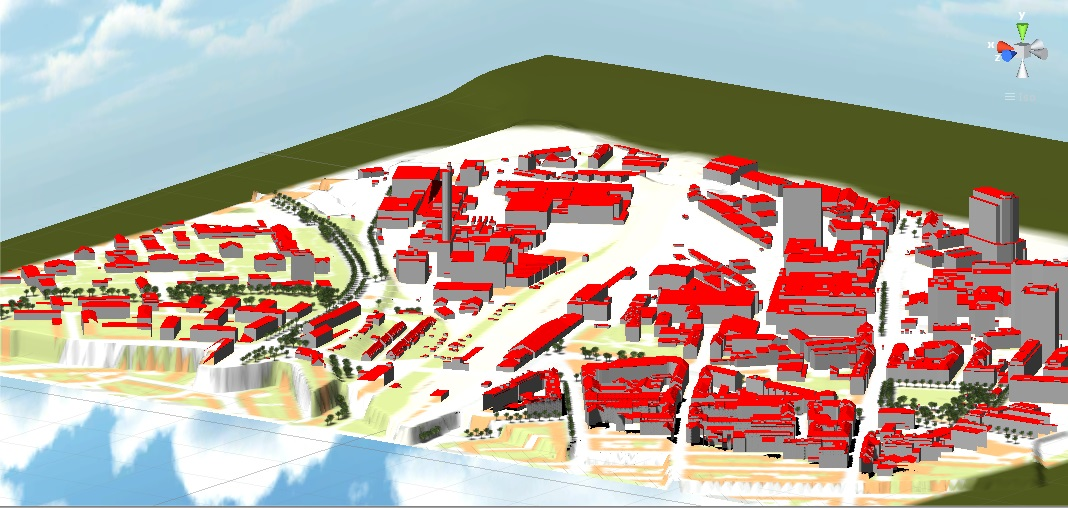
\includegraphics[width=0.8\textwidth]{unity}
\vspace{0.5cm}
\begin{Large}
Departement Mathematik und Informatik\\
\end{Large}
High-Performance and Web Computing\\
http://informatik.unibas.ch/\\
\vspace{0.5cm}
\begin{tabular}{llll}
{\bf Autor} & Maurus Dähler & {\bf Betreuer} & Dr. Martin Guggisberg\\
{\bf E-Mail} & m.daehler@stud.unibas.ch & {\bf Prüfer} & Prof. Helmar Burkhart\\
{\bf Matr.-Nr.} & 09-053-547\\
\end{tabular}


25.08.2014\\
\vspace{0.5cm}

\includegraphics[width=0.1\textwidth]{unisignet}


\end{center}
\clearpage


\pagestyle{useheadings} % normale Kopf- und Fußzeilen für den Rest
\renewcommand{\baselinestretch}{1.5}\normalsize

\tableofcontents
\listoffigures

\chapter*{Abk\"urzungen}\label{c.abk}
\vspace{-20pt}
\addcontentsline{toc}{chapter}{Abk\"urzungen}
\markboth{Abk\"urzungen}{Abk\"urzungen}
\begin{flushleft}\begin{tabularx}{\textwidth}{l|X}
Abk\"urzung & Bedeutung\\\hline
AR & Augmented Reality: Einblenden digitaler Inhalte in die reale Welt\\
DGPS & Differential Global Positioning System: Verfeinertes GPS Systems, welches eine Abweichung von wenigen Zentimetern bietet\\
DOF & Degrees of Freedom: Anzahl Freiheitsgrade bzw. Bewegungsrichtungen, welche ein Sensor erkennen kann\\
FOV & Field of View: Das Sichtfeld der Kamera bzw. des Auges\\
HMD & Head Mounted Display: Bildschirmsystem, welches direkt vor den Augen auf dem Kopf montiert wird\\
SBAS & Satellite Based Augmentation System: Positionserkennung mithilfe geostationärer Satelitten\\
VR & Virtual Reality: gänzlich von einem Computer generierte Welt, in welcher man sich bewegen kann\\
\end{tabularx}\end{flushleft}


\chapter{Einleitung}
\vspace{-20pt}
\pagenumbering{arabic} % ab jetzt die normale arabische Nummerierung
Diese Arbeit soll einerseits einen Überblick über Technologien in virtueller und augmentierter Realität bieten und anderseits das erstellte Pilotprojekt vorstellen. Die Resultate sollen in das Forschungsprojekt HUVis (Handheld Urban Visualization) einfliessen.\\[6pt]
Nach einer kurzen Einführung in die Grundlagen von VR/AR und ausgewählter Projekte, wie z.B. das in Zusammenarbeit mit der \textit{Fachhochschule Nordwestschweiz}, \textit{i-art interactive AG} und der \textit{Universität Basel} entwickelte \textit{LifeClipper2}, wird auf verschiedene Hardwaresysteme eingegangen. Es werden die diverse Bildschirmtechnologien mit einem verstärkten Fokus auf Head Mounted Displays (HMD) vorgestellt, da diese die höchste immersive Erfahrung bieten. Hier soll der \textit{Oculus Rift} besonders beachtet werden, da dieser für das Softwareprojekt eingesetzt wurde. Des Weiteren werden in diesem Kapitel akustische und haptische Ausgabegeräte und diverse Positionsbestimmungsmethoden, welche für AR Anwendungen wichtig sein werden, betrachtet.\\[6pt]
Im zweiten Teil der Arbeit wird das Pilotprojekt, in welchem eine VR Erfahrung des St. Johann Quartiers in Basel entwickelt wurde, beschrieben. Für das Erstellen der Bodentexturierung konnte mithilfe des selbst entworfenen Programms \textit{TileGrabber} eine Karte des Gebiets aus hochauflösenden Kartenausschnitten automatisiert zusammengestellt werden. Anschliessend folgen Überlegungen, wie das Projekt in einer nächsten Phase zu einer augmented Reality Erfahrung weiterentwickelt werden kann. Im letzten Kapitel werden schliesslich exemplarisch die Möglichkeiten der \textit{Unity} Engine vorgestellt.

\chapter{Hintergründe zu Virtual und Augmented Reality}\label{c.wasist}
\vspace{-20pt}
\section{Virtual Reality}
Ziel eines VR Systems ist es den Betrachter vollständig in die vom Computer erschaffen Welt einzubringen. Sie wird bereits seit mehreren Jahren für Produktentwicklungen sowie vielen Industriebranche, wie Automobilhersteller, Architekten oder das Militär, als Werkzeug genutzt. Durch die vorangeschrittene Entwicklung in der Displaytechnologie konnten die Systeme immer günstiger produziert und verkauft werden. Somit sind sie nun für Privatverbraucher erschwinglich. Doch ob es sich nun um einfache Head Mounted Displays handelt oder visionäre Systeme wie das Holodeck aus Star Treck (ein Raum, welcher sich den Gedanken des Nutzers anpasst), wird VR durch folgende Definitionen äusserst treffend beschrieben.
\begin{quote}
''Virtual Reality (VR) refers to the use of three-dimensional displays and interaction devices to explore real-time computer generated environments.''\\
(Steve Bryson, Call for Participation 1993 IEEE Symposium on Research Frontiers in Virtual Reality)

''Virtual Reality refers to immersiv, interactive, multi-sensory, viewer-centered, three-dimensional computer generated environments and the combination of technologies requiered to build these environments.''\\
(Carolina Cruz-Neira, SIGGRAPH '93 Course Notes ''Virtual Reality Overview'')
\end{quote}
Ziel von VR ist es somit 3D-Inhalte des Computers nicht über den zweidimensionalen Display wahrzunehmen, sondern mithilfe von stereoskopischen Displays die Inhalte räumlich darzustellen. Hinzu kommt das Ansprechen weiterer Sinne wie Hör- und Tastsinn. Bei der Umsetzung eines solchen Systems möchte man einen hohen Grad an Immersion erreichen. Nach Slater und Wilbur \cite[S.~5~ff.]{slaterwilbur97} müssen Ausgabegeräte für Immersion folgende vier Eigenschaften besitzen
\begin{enumerate}\itemsep1pt \parskip0pt \parsep0pt
	\item Sinneseindrücke des Menschen sollen möglichst ausschliesslich durch den Computer generiert werden, d.h. der Nutzer soll weitestgehend von der realen Umgebung isoliert werden
	\item möglichst viele Sinne sollen angesprochen werden
	\item die Ausgabegeräte sollen den Nutzer vollständig umgeben, anstatt nur ein enges Sichtfeld zu bieten
	\item zudem sollen die Ausgabegeräte eine ''lebendige'' Darstellung bieten, z.B. durch hohe Auflösung und Qualität der Farbdarstellung
\end{enumerate}
Somit stellen geschlossene HMDs, welche das Sichtfeld des Nutzers umschliessen und es ihm nur noch ermöglichen die virtuellen Inhalte zu sehen, höchst immersive Displays dar.\cite[S.~12~ff.]{doerner13}\\[6pt]

\section{Augmented Reality}
In manchen Bereichen ist es nicht nötig oder erwünscht eine komplette virtuelle Welt zu betrachten, sondern nur ein virtuelles Objekt in die reale Welt einzufügen. Mithilfe von Augmented Reality ist dies möglich. Eine passende Definition findet sich in \cite{doerner13}.
\begin{quote}
Unter Augmentierter Realität [...] versteht man allgemein die Anreicherung der Realität durch künstliche virtuelle Inhalte. Dabei kommt es zu einer Verschmelzung der Realität mit der Virtualität.
\end{quote}
Grundsätzlich müssen bei AR fünf Arbeitsschritte ausgeführt werden: Videoaufnahme, Tracking, Registrierung, Darstellung und Ausgabe.\\[6pt]  
Die Videoaufnahme entfällt, falls es sich um ein optisches See-Through-AR System handelt, siehe dazu Kapitel \ref{s.formen}. Ansonsten wird das Videobild genutzt, um später die digitalen Inhalte darüberzulegen.\\[6pt]   
Beim Tracking wird die Position und Orientierung des Betrachters erfasst, damit eine perspektivisch korrekte Darstellung der Inhalte erfolgt. Zur Orientierungsbestimmung können 3-DOF Sensoren eingesetzt werden. Die genaue Position in einem grösseren Massstab zu bestimmen ist hingegen schwierig, in Kapitel \ref{c.hardware} wird genauer auf die Schwierigkeiten eingegangen und die Funktionsweise von 3-DOF bzw. 6-DOF Sensoren beschrieben.\\[6pt]  
 Bei der Registrierung werden die gewonnen Informationen aus dem Tracking so genutzt, dass die digitalen Inhalte in der Realität verankert erscheinen. Dies führt dazu, dass das Objekt an seinem zuvor definierten Punkt in der realen Welt bleibt, auch wenn die Position des Betrachters verändert wird. 
 Im Darstellungsschritt werden schliesslich die digitalen Inhalte der Videoaufnahme hinzugefügt und gegebenenfalls angepasst um perspektivische Korrektheit zu gewährleisten.\\[6pt]  
 Schlussendlich erfolgt die Ausgabe des augmentierten Bildes. Dies kann auf jeglicher Art Display erfolgen, für höchste Immersion sind jedoch HMDs zu bevorzugen.\cite[S.~241~ff.]{doerner13}

\chapter{Übersicht ausgewählter VR/AR Projekte}\label{c.projects}
\vspace{-20pt}
\section{LifeClipper2}\label{s.clipper}
\textit{LifeClipper2} ist ein in Zusammenarbeit mit der \textit{Fachhochschule Nordwestschweiz}, \textit{i-art interactiv AG} und der \textit{Universität Basel} entwickeltes AR Forschungsprojekt. Es beinhaltet vier Szenarien, mit welchen es dem Anwender möglich ist die Entwicklung des St. Johann Quartiers als AR Erfahrung zu erleben. Mithilfe eines virtuellen Lifts ist es möglich das Gebiet aus grosser Höhe zu betrachten. Da der Nutzer selbst, und somit sein Blickfeld, am Boden bleibt findet ein Wechsel von augmentierterter zu virtueller Realität statt. Zudem ist es möglich die Resultate grösserer Bauprojekte bereits als Augmentierung zu betrachten. Im Gegensatz zu vorgefertigten Videosimulationen oder Bildern ist die Erfahrung um einiges realer \cite[S.~172~ff.]{website:lifeclipper}\\[6pt]

\begin{figure}[ht]
	\vspace{-15pt}
	\begin{center}
		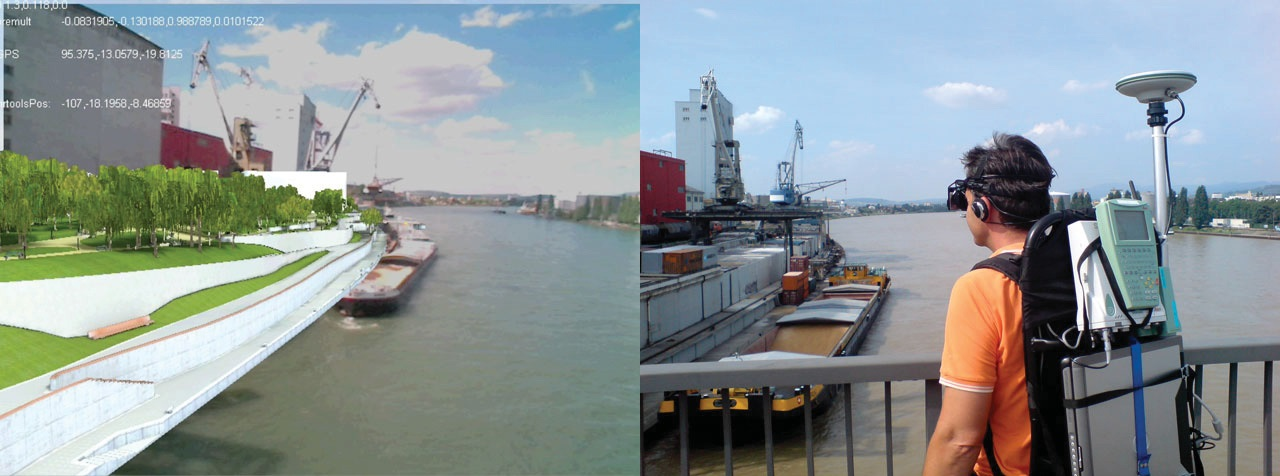
\includegraphics[width=0.9\textwidth]{lifeclipper}
	\end{center}
	\vspace{-15pt}
	\caption[LifeClipper2 im Einsatz]{LifeClipper2 im Einsatz: Rechts das augmentierte Bild des Systems, links ein Bild des Anwenders}\label{lifeclipper}
	\vspace{-10pt}
\end{figure}


\section{Schweissmaske der Zukunft}\label{s.welding}
Moderne Schweissmasken erkennen, wann das Schweissen beginnt und verdunkeln das Visier um die Augen des Anwenders zu schützen. Es ist jedoch äusserst schwierig die Spitze des Schweissgerätes mit verdunkeltem Visier zu sehen, was nötig wäre um präzise schweissen zu können. Mithilfe von High Dynamic Range Kameras kann die Szene aufgenommen und korrigiert werden. Dunkle Stellen werden aufgehellt, helle hingegen abgedunkelt. Dies geschieht mit einem Kontrastverhältnis von 100'000'000:1. Ein Wert, welcher weit über den menschlichen Wahrnehmungsfähigkeiten liegt.\\[6pt]

\vspace{-30pt}
\begin{figure}[h]%
	\centering
	\subfigure[][]{%
	\label{weldingaug}%
	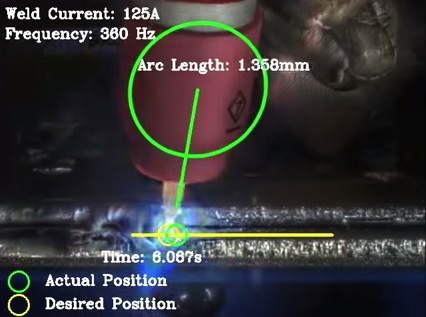
\includegraphics[width=0.46\textwidth]{weldingaug}}%
	\hspace{8pt}%
	\subfigure[][]{%
	\label{welding}%
	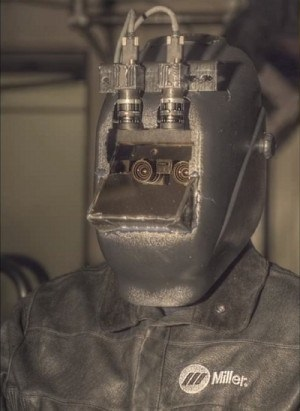
\includegraphics[width=0.25\textwidth]{welding}}%
	\caption[Schweissmaske der Zukunft]
	{Schweissmaske der Zukunft:
	\subref{fig:see-a} Augmentierungen während des Schweissens,
	\subref{fig:see-b} Aussehen der Schweissmaske}%
	\label{fig:weld}%
\end{figure}
\vspace{-15pt}
Resultat dieser Aufnahme- und Bearbeitungsart ist, dass beim Schweissen lediglich ein weisser Punkt an der Spitze der Schweissnadel zu sehen ist und der Rest der Szenerie völlig normal beleuchtet wird. Daneben ist es auch möglich weitere Augmentierungen, welche nützliche Informationen für den Anwender liefern, einzublenden. So zum Beispiel eine gelbe Linie, nach der man sich richten kann, welche sich rot färbt sobald man davon abweicht oder der Abstand zwischen der Schweissnadel und dem Metallstück zu klein oder zu gross ist.\cite{website:welding}

\newpage
\section{Panzer aus Glas}\label{s.tank}
\begin{wrapfigure}{r}{0.5\textwidth}
	\vspace{-25pt}
	\begin{center}
		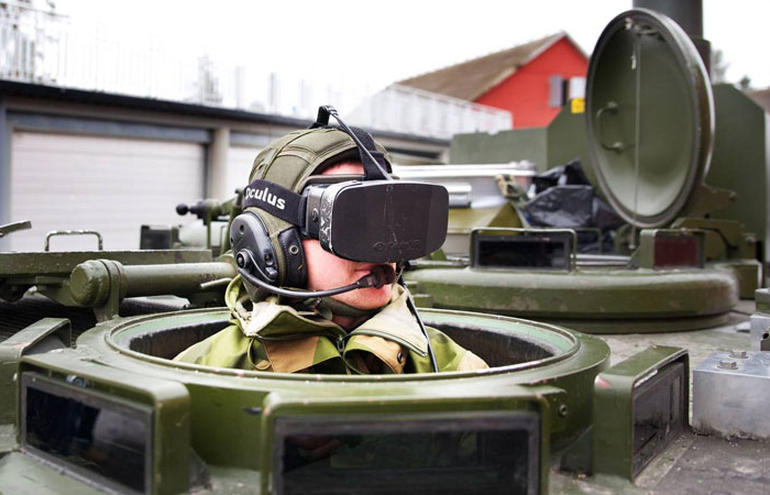
\includegraphics[width=0.45\textwidth]{tank}
	\end{center}
	\vspace{-15pt}
	\captionsetup{width=0.42\textwidth}
	\caption{Norwegischer Panzersoldat mit \textit{Oculus Rift}}\label{tank}
	\vspace{-10pt}
\end{wrapfigure}
In Norwegen wird beim Militär zur Zeit ein AR System für Panzerfahrer mithilfe des \textit{Oculus Rift} getestet. Das System besteht aus vier Kameras, welche mit einem Sichtfeld (auch FOV, field of view, genannt) von 185\textdegree eine 360\textdegree-Sicht um den Panzer herum ermöglichen. Diese Bilder werden anschliessend genutzt um der Besatzung des Panzers durch den \textit{Oculus} eine freie Sicht auf das geschehen Ausserhalb zu ermöglichen. Da jedoch Ausrüstung, welche ausserhalb des Panzers angebracht wird, sich in einer Gefahrenzone befindet (entweder durch Direktfeuer oder Schrapnell) kann das System noch nicht vollständig integriert werden.\cite{website:tank}
\vspace{-12pt}
\section{AR für Blinde}\label{s.shoes}
\begin{wrapfigure}{r}{0.5\textwidth}
	\vspace{-65pt}
	\begin{center}
		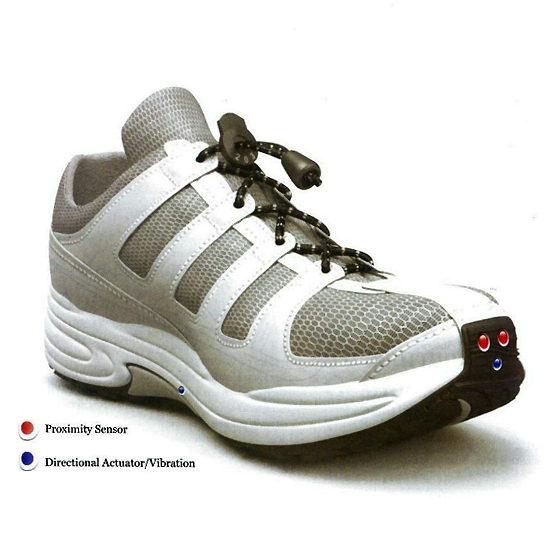
\includegraphics[width=0.45\textwidth]{shoes}
	\end{center}
	\vspace{-15pt}
	\captionsetup{width=0.42\textwidth}
	\caption{\textit{Le Chal}: Der sehende Schuh}\label{shoes}
	\vspace{-10pt}
\end{wrapfigure}
Der in Indien entwickelte haptische Schuh kann mit einem beliebigen Smartphone über Bluetooth gekoppelt werden. Nach der Routeneingabe im Navigationsapp des Smartphones teilt der Schuh mithilfe von Vibrationen mit, ob der Nutzer nach links, rechts oder geradeaus zu laufen hat. Zudem befindet sich an der Spitze des Schuhs ein Annäherungssensor, welcher den Anwender vor Hindernissen warnt. Für Menschen mit eingeschränkter Sicht ist es so möglich, sich frei und ohne andere Hilfsmittel wie Blindenstock oder Blindenhund zu bewegen.\cite{website:shoes}

\chapter{State of the art VR/AR-Technologie}\label{c.hardware}
\vspace{-20pt}
\section{Formen von AR}\label{s.formen}
Im Bereich der AR unterscheidet man zwischen drei grundlegenden Formen der Umsetzung. Video und optische See-Through Systeme sowie projektorientierte AR. Je nach Anforderung an das System haben diese Formen Vor- und Nachteile vorzuweisen. Es ist ihnen jedoch gemein, dass sie die digitalen Inhalte in perspektivisch korrekter Form darstellen sollen. Somit muss eine Übereinstimmung der digitalen und realen Blickrichtung gegeben sein und das virtuelle Blickfeld muss dem tatsächlichen entsprechen.\cite[S.~247]{doerner13}
\subsection*{Video See-Through-AR}
\begin{wrapfigure}{r}{0.5\textwidth}
	\vspace{-20pt}
	\begin{center}
		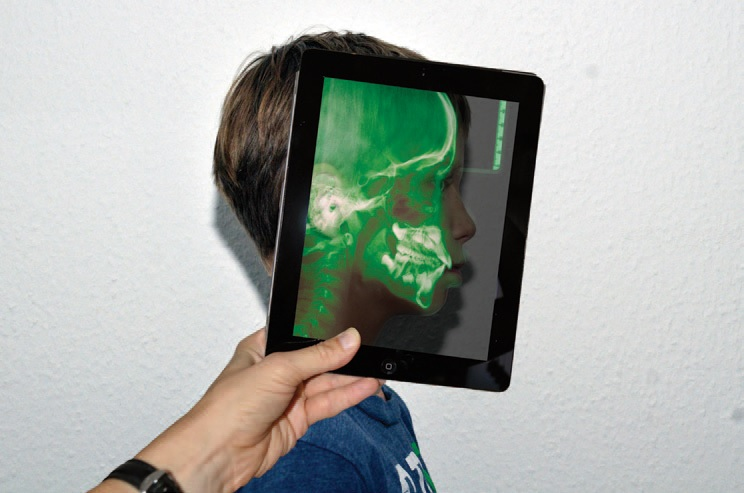
\includegraphics[width=0.45\textwidth]{magiclens}
	\end{center}
	\vspace{-15pt}
	\caption{Magic-Lens-Effekt}\label{magiclens}
	\vspace{-10pt}
\end{wrapfigure}
Bei der Video See-Through-AR Methode wird über eine oder mehrere Kameras die reale Welt aufgenommen. Anschliessend werden die digitalen Inhalte hinzugefügt und an den Display zurückgesendet. Um eine Übereinstimmung der realen und virtuellen Blickrichtung sowie des Blickfelds zu erreichen, müssen die Positionen der Kameras in der Realität mit der Position der digitalen Kamera in der Simulation übereinstimmen, siehe Kapitel \ref{s.positional}. Ansonsten führt dies zu einer Fehlplatzierung des digitalen Objekts. Bei der korrekten Ausrichtung beider Kameras tritt der sogenannte Magic-Lens-Effekt auf, bei welchem es scheint als ob man durch eine Scheibe die veränderte Realität beobachtet, siehe Abbildung \ref{magiclens}.\cite[S.~248]{doerner13}.

\begin{wrapfigure}{l}{0.6\textwidth}
	\vspace{-20pt}
	\begin{center}
		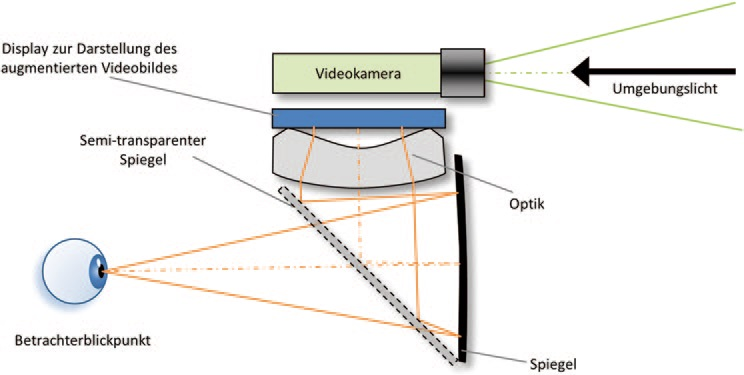
\includegraphics[width=0.55\textwidth]{videoseewrongpos}
	\end{center}
	\vspace{-15pt}
	\captionsetup{width=0.5\textwidth}
	\caption{Beispielaufbau Video See-Through-AR}\label{videoseewrongpos}
	\vspace{-10pt}
\end{wrapfigure}
Video-See-Through-Displays sind grundsätzlich Datenbrillen mit einer oder mehreren Kameras, welche auch für VR Anwendungen genutzt werden können. Es können auch Smartphones und Tablets dafür verwendet werden, in dieser Arbeit wird jedoch nicht weiter darauf eingegangen da sie keinen hohen Grad an Immersion ermöglichen. Die Kameras sollten über ein grösseres Blickfeld als die Datenbrille verfügen, da das Anbringen der Kameras im Strahlengang, welcher direkt vor den Augen liegt, meist nicht möglich ist. Deshalb wird eine perspektivische Korrektur der Videoinhalte nötig. Sollte es möglich sein die Linse der Kamera direkt vor dem Auge anzubringen bzw. mithilfe von Spiegeln das eingehende Licht umzuleiten, ist diese Korrektur nicht mehr nötig.\cite[S.~271 ff.]{doerner13}\\[6pt]
Vorteil eines solchen Systems ist wie schon erwähnt die Möglichkeit es als VR Lösung einzusetzen. Die Nachteile liegen insbesondere bei dem höheren Rechenaufwand, da neben dem digitalen Inhalt auch das Videobild der Kamera verarbeitet werden muss. Ausserdem wird durch das Anbringen von Kameras an dem HMD das System, im Gegensatz zu optischen See-Through-AR, relativ gross und schwer.
\newpage
\subsection*{Optisches See-Through-AR}
\begin{wrapfigure}{r}{0.35\textwidth}
	\vspace{-20pt}
	\begin{center}
		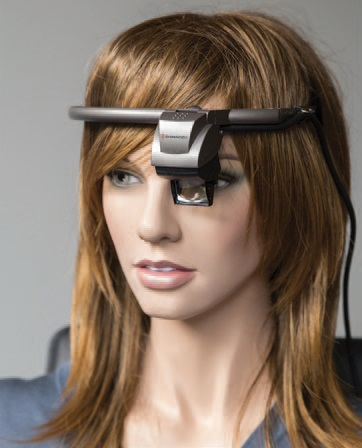
\includegraphics[width=0.32\textwidth]{opticseehmd}
	\end{center}
	\vspace{-15pt}
	\captionsetup{width=0.3\textwidth}
	\caption{Beispiel eines optischen See-Through HMD}\label{optseehmd}
	\vspace{-10pt}
\end{wrapfigure}
Mithilfe semitransparenter Displays ist bei der optischen See-Through-AR Methode die Aufnahme der Realität mithilfe von Kameras nicht nötig, kann jedoch zur Positionsbestimmung vorhanden sein. Wie schon bei der Video See-Through-AR Methode muss die Perspektive des realen Umfelds und der virtuellen Inhalte übereinstimmen. Dazu muss der Blickpunkt relativ zum Display bekannt sein. Es ist daher nötig, dass für jedes Auge ein separater Display verwenden werden muss. Mit einem stereoskopischen Display ist es jedoch möglich, dass beide Augen denselben Display betrachten.\cite[S.~248~f.]{doerner13}\\[6pt]
Im Aufbau gibt es verschiedene Ansätze. Allen ist jedoch gemein, dass sie die reale Umgebung lediglich mit den virtuellen Inhalten optisch überlagern. Dadurch findet, im Gegensatz zur Video-See-Throug Methode, kein Qualitätsverlust bei der Wahrnehmung der Realität statt. Es ist nicht mehr möglich Objekte der Realität vollständig auszublenden oder zu überdecken. Durch die Überlagerung findet des weiteren eine Reduktion der einfallenden Lichtmenge statt und wegen der geringen Lichtstärke der meisten HMD dieser Art ist eine Anwendung bei Sonnenlicht kaum möglich.\\[6pt]
Die gängigste Bauweise verwendet semi-transparente Spiegel. Die digitalen Inhalte werden über zwei Spiegel zum Auge umgeleitet. Diese lassen jeweils einen Teil des Lichts passieren und reflektieren einen anderen Teil. Dadurch wird die Helligkeit des Umgebungslichts als auch des Displays reduziert. Mithilfe von Prismen versucht man diesen Helligkeitsverlust zu reduzieren. Da ein einzelnes Prisma, welches die digitalen Inhalte zum Auge leitet, auch die einfallenden Lichtstrahlen der Umgebung beeinflussen würde, muss ein zweites Prisma verwendet werden um diese Krümmung zu korrigieren. Retinale Datenbrillen hingegen projizieren die digitalen Inhalte direkt auf die Retina. Dadurch sind sehr kompakte Bauweisen mit grossen Blickfeldern möglich und es entfällt eine aufwändige Optik, durch die sich das Auge auf die digitalen Inhalte fokussieren kann. Es wird zumeist moduliertes Laserlicht, welches über semi-transparente Spiegel oder ein Prisma zum Auge geleitet wird, verwendet.\\[6pt]

\subfiglabelskip=0pt
\begin{figure}[h]%
	\centering
	\subfigure[][]{%
		\label{fig:see-a}%
		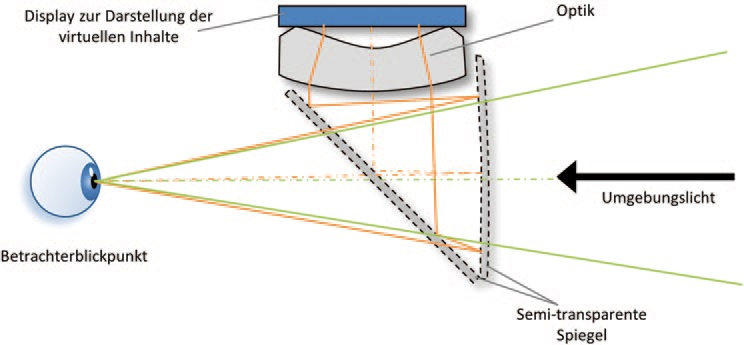
\includegraphics[width=0.45\textwidth]{opticseemir}}%
	\hspace{8pt}%
	\subfigure[][]{%
		\label{fig:see-b}%
		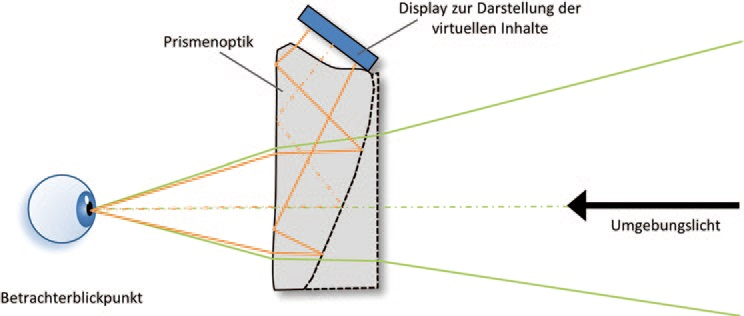
\includegraphics[width=0.45\textwidth]{opticseepris}}%
	
	\subfigure[][]{%
		\label{fig:see-c}%
		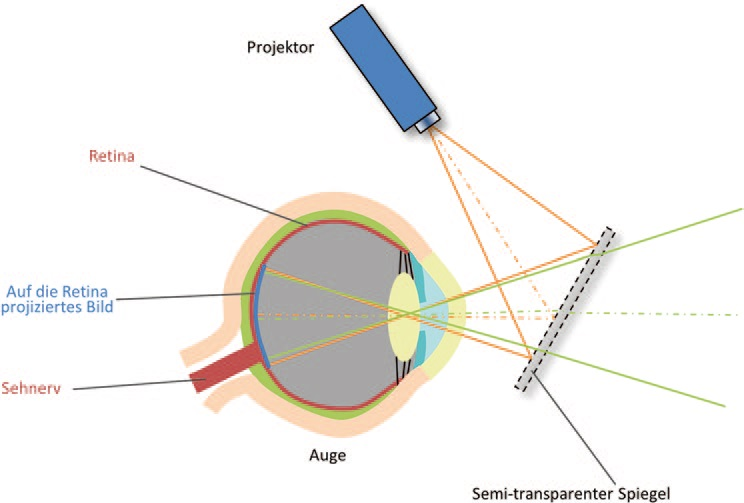
\includegraphics[width=0.4\textwidth]{opticseeretina}}%
	\hspace{8pt}%
	\subfigure[][]{%
		\label{fig:see-d}%
		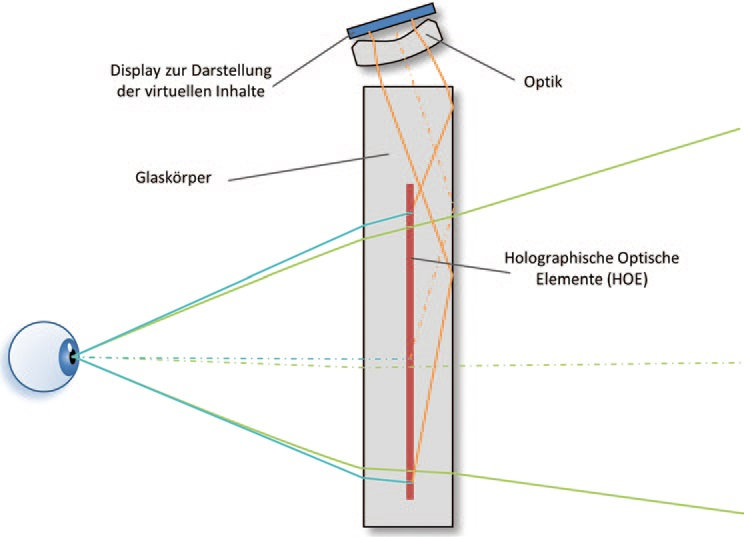
\includegraphics[width=0.4\textwidth]{opticseehoe}}%
	\caption[Bauweisen für See-Through Systeme.]
	{Bauweisen für optische See-Through Systeme:
		\subref{fig:see-a} semi-transparente Spiegel,
		\subref{fig:see-b} prismenbasiertes Display,
		\subref{fig:see-c} Retinale Datenbrille, und
		\subref{fig:see-d} optische Elemente.}%
	\label{fig:see}%
\end{figure}
Eine weitere Möglichkeit ist das integrierte optische Elemente an. Hierbei wird Licht im Inneren eines planaren Glaskörpers so umgeleitet, dass es ins Auge reflektiert wird. D.h. das digitale Bild wird seitlich oder von oben in die Glasscheibe eingespiesen und tritt vor dem Auge wieder aus. Dies erlaubt eine relativ flache Bauweise des Displays und so konstruierte Datenbrillen können stark an normale Sonnenbrillen erinnern.\cite[S.~273~ff.]{doerner13}
\newpage
\subsection*{Projektionsbasierte AR}
\begin{wrapfigure}{r}{0.45\textwidth}
	\vspace{-25pt}
	\begin{center}
		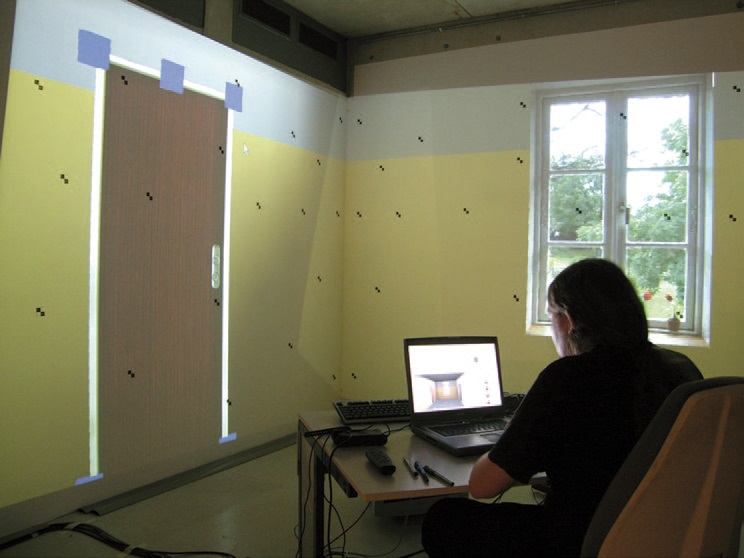
\includegraphics[width=0.4\textwidth]{projsee}
	\end{center}
	\vspace{-15pt}
	\captionsetup{width=0.38\textwidth}
	\caption{Beispiel einer projektionsbasierten AR}\label{projsee}
	\vspace{-15pt}
\end{wrapfigure}
Die projektionsbasierte AR Methode verwendet im Gegensatz zu den zuvor vorgestellten Methoden keinen Display zur Darstellung der Augmentierung. Hier werden mit Hilfe von Projektoren Oberflächeneigenschaften manipuliert oder zusätzliche Informationen dargestellt.\cite[S.~249]{doerner13}\\[6pt]
Mobile Anwendungen sind wegen der benötigten Oberflächen zur Darstellung der Augmentierung daher kaum zu realisieren. Ausserdem ist durch die geringe Helligkeit aktueller Projektoren eine Anwendung im Freien bei Sonnenlicht nicht vorstellbar. Deshalb wird im Rahmen dieser Arbeit, bis auf die Vorstellung eines projektionsbasierten HMD im Kapitel \ref{s.displays}, auf diese Methode nicht weiter eingegangen.\\[6pt]
\newpage

\section{Head Mounted Displays}\label{s.displays}
\subsection*{Allgemein}
Durch das erhöhte Interesse an VR/AR wurden in den letzten Monaten mehrere neue Systeme entwickelt, welche bereits im Handel verfügbar oder als Developer Version für Tests erhältlich sind. In diesem Abschnitt wird eine Auswahl dieser Systeme vorgestellt, mit welchen sich Outdoor-AR-Anwendungen realisieren lassen.\\[6pt]
Die wichtigste Kenngrösse von HMDs ist ihr Field of View. Dieser beschreibt den horizontalen und vertikalen Winkel ausgehend vom Auge, von welchem die virtuellen Informationen wahrgenommen werden. Je grösser das FOV umso immersiver ist die VR Erfahrung. Für Video See-Through-AR Systeme ist es deshalb wichtig Kameras mit Weitwinkelobjektiven zu verwenden, da ansonsten der FOV bereits durch die Kameras eingeschränkt wird. Bei optischen See-Through-AR Systemen wird mithilfe des FOV hingegen die Einschränkung der Sicht durch das System beschrieben (z.B. vorhandene Ränder der Brille, welche die Sicht verdecken).\cite[S.~142~ff.]{doerner13}\\[6pt]
\vspace{-15pt}
\begin{wrapfigure}{r}{0.5\textwidth}
	\vspace{-25pt}
	\begin{center}
		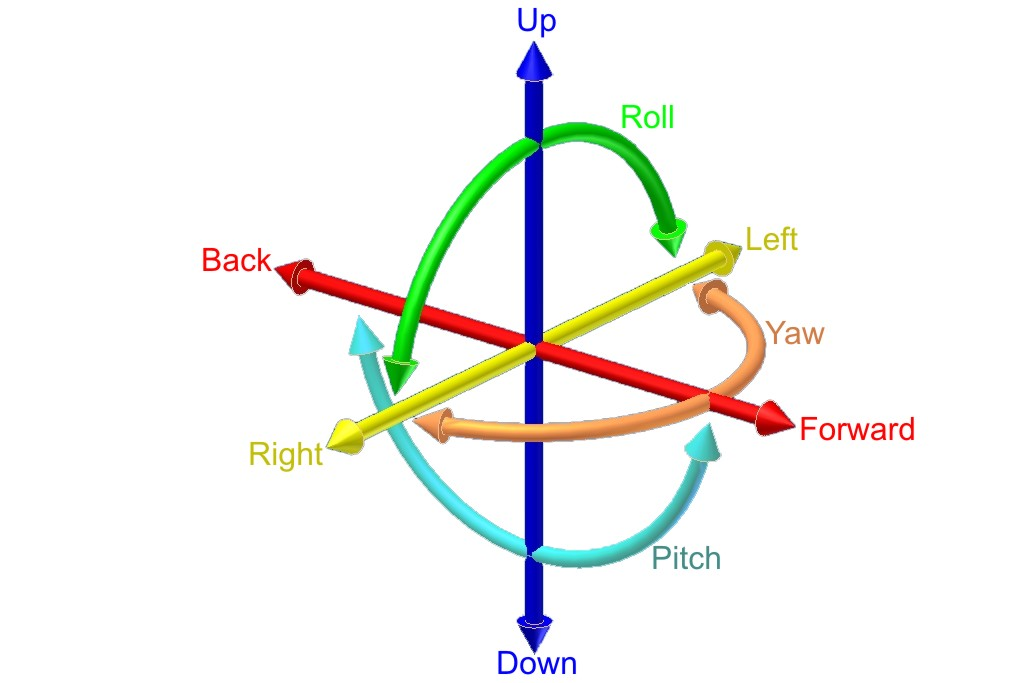
\includegraphics[width=0.45\textwidth]{6DOF_en}
	\end{center}
	\vspace{-15pt}
	\captionsetup{width=0.42\textwidth}
	\caption{Die sechs erkennbaren Lageänderungen eins 6-DOF Sensors}\label{dof}
	\label{fig.dof}
	\vspace{-10pt}
\end{wrapfigure}
 In der Regel ist ein 3-DOF Sensor, welcher aus einem Gyroskop (Kreiselinstrument) oder Accelerometer (Beschleunigungssensor) besteht, zur Orientierungsbestimmung im HMD eingebaut. DOF (Degress of Freedom) bedeutet Freiheitsgrade. In diesem Fall beschreibt es die Anzahl Orientierungen, welche der Sensor aufnehmen kann. Ein 3-DOF Sensor kann drei unterschiedliche Orientierungsänderungen erkennen. Ist ein Gyroskop verbaut, wie in HMDs üblich, können die in Abbildung \ref{fig.dof} als Roll (Rollen), Pitch (Neigen) und Yaw (Schwenken) bezeichneten Bewegungen erkannt werden. Diese Begriffe sind auch in der Aviatik zur Beschreibung von Flugbewegungen gebräuchlich. Rollen und Neigen können mithilfe der auf die im Gyroskop eingebauten Kreisel einwirkenden Gravitationskräfte zu Beginn bestimmt werden. Die Auslenkung in der Schwenkbewegung wird im Initialstadium gemessen und so angenommen, dass sie dem Blick nach vorne entspricht. Anschliessend ist es möglich die Änderung der Blickrichtung des Nutzers zu erkennen und an die VR/AR-Applikation weiterzuleiten um die digitale Kamera neu auszurichten. Möchte man Bewegung im Raum, wenn der Nutzer zum Beispiel einen Schritt nach vorne macht, erkennen, müssen sowohl Gyroskop als auch Accelerometer vorhanden sein. Durch kombinieren der gewonnen Daten kann auf die Richtung und die zurückgelegte Distanz geschlossen werden. In diesem Fall spricht man von 6-DOF Sensoren.\cite{website:dof}
\subsection*{Vuzix Wrap 1200DXAR}
\begin{wrapfigure}{r}{0.5\textwidth}
	\vspace{-20pt}
	\begin{center}
		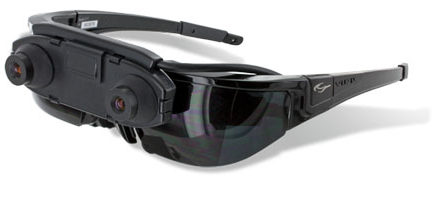
\includegraphics[width=0.45\textwidth]{1200dxar-full}
	\end{center}
	\vspace{-15pt}
	\caption{\textit{Vuzix Wrap 1200DXAR}}\label{vuzixgraphic}
	\vspace{-12pt}
\end{wrapfigure}
Die Firma Vuzix stellt schon seit einigen Jahren Videobrillen zum Betrachten von Multimediainhalten her. Bei der \textit{Wrap 1200DXAR} handelt es sich um ein Video See-Through-AR System, siehe Kapitel \ref{s.formen}. Die Brille verfügt über zwei Kameras, welche das Bild in VGA Qualität aufnehmen, einen 3-DOF Sensor um die Lage der Brille zu bestimmen, In-Ear Headphones und zwei LCD Displays. Des weiteren ist es möglich den Fokus der beiden Displays für Brillenträger zwischen +2 und -3 Dioptrien einzustellen, was das Tragen einer korrigierten Brille oder Kontaktlinsen erübrigt. AR Anwendungen können mithilfe des zur Verf"ugung gestellten SDK für Windows programmiert werden. Das AR System unterstützt neben Windows keine weiteren Betriebssysteme. Durch die leichte Bauform und das Sonnenbrillendesign ist eine Anwendung im Alltag vorstellbar. Aufgrund der eher auffälligen Stereokamera sollte man sich jedoch auf verwunderte Blicke gefasst machen. \cite{website:vuzix}
\newpage
\subsection*{Epson Moverio BT-200}
\begin{wrapfigure}{l}{0.5\textwidth}
	\vspace{-20pt}
	\begin{center}
		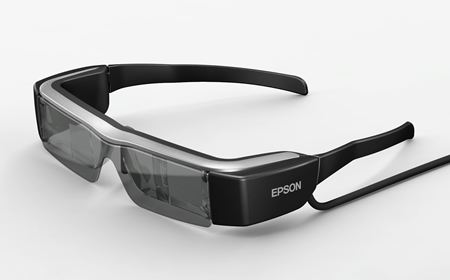
\includegraphics[width=0.45\textwidth]{moverio_unique}
	\end{center}
	\vspace{-15pt}
	\caption{\textit{Epson Moverio BT-200}}\label{moveriogrpahic}
	\vspace{-12pt}
\end{wrapfigure}
Bei der Moverio handelt es sich um ein optisches See-Throug-AR System, welches Android als Betriebssystem verwendet. Anders als die zuvor erwähnte \textit{Vuzix} ist somit ein externes System in Form eines Computers oder Laptops, welcher die AR Applikation ausführt und das Bild zu der Brille sendet, nicht nötig. Es ist jedoch zu beachten, dass durch die geringe Leistung der Hardware die graphische Qualität der virtuellen Inhalte eher bescheiden ist.  Sie besitzt wie auch die \textit{Vuzix} über einen 3-DOF Sensor zur Bestimmung der Kopflage. Ausserdem sind ein GPS Sensor und ein Kompass in die Brille integriert und sie ist somit die einzige hier vorgestellte Brille, die im weiteren Sinne einen 6-DOF Sensor besitzt. Damit ist gemeint, dass der Sensor nicht über einen konventionellen Accelerometer verfügt um die Bewegung im Raum zu erkennen sondern mithilfe von GPS die Position bestimmt. Zudem besitzt sie  ein Mikrofon, mit welchem Applikationen per Sprachbefehl gesteuert werden können. Da mittels des semi-transparent Displays die Kameras im Gegensatz zur zuvor vorgestellten \textit{Vuzix} entfallen, ist ein Tragen der Brille im Alltag eher vorstellbar.\cite{website:epson}
\newpage
\subsection*{castAR}
\begin{wrapfigure}{r}{0.4\textwidth}
	\vspace{-30pt}
	\begin{center}
		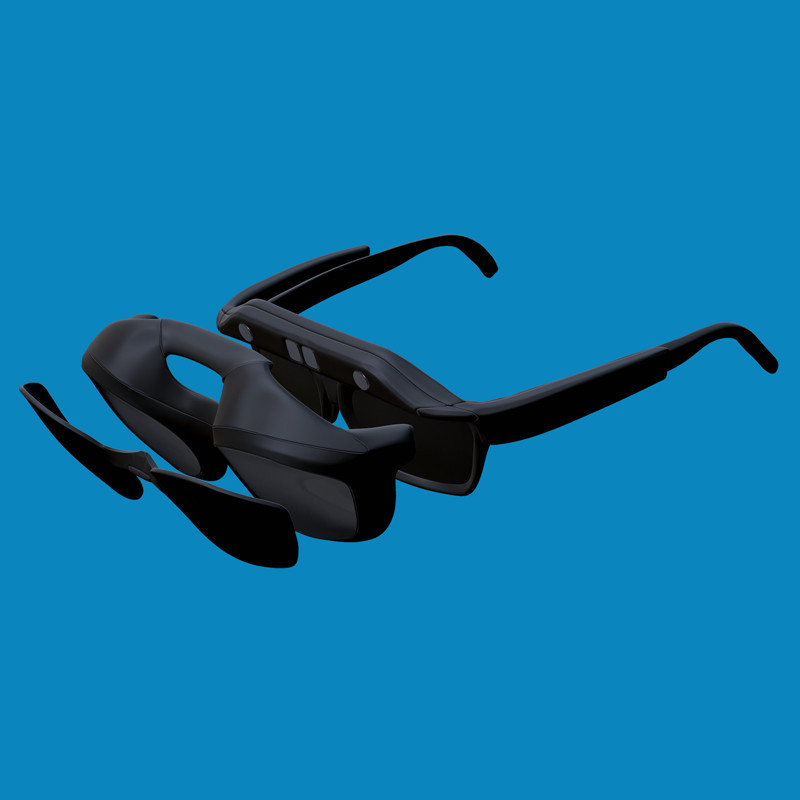
\includegraphics[width=0.35\textwidth]{castAR}
	\end{center}
	\vspace{-15pt}
	\captionsetup{width=0.32\textwidth}
	\caption{\textit{castAR} mit optionalem mobil AR Clip-On}\label{castAR}
	\vspace{-15pt}
\end{wrapfigure}
Ein gänzlich anderer Ansatz kommt von der Firma Technical Illusions. Bei der von Technical Illusions entwickelten Brille handelt es sich um ein projektionsbasiertes AR System. Die Brille verfügt über zwei Projektoren, welche das Bild auf die Oberfläche vor dem Nutzer projizieren. Die polarisierten Gläser der Brille fügen die beiden Teilbilder anschliessend, ähnlich wie bei 3D-Kino Brillen, zu einem einzigen dreidimensionalen Bild zusammen. Des Weiteren verfügt sie über eine hochauflösende Kamera, um die absolute Kopfposition zu bestimmen und einen 3-DOF Sensor zur Bestimmung der Blickrichtung. Ausserdem wird in naher Zukunft ein Zusatz angeboten werden, welcher auf die vorhande Brille geklipt werden kann. Dieser reflektiert die Ausgabe der Projektoren direkt vor den Augen, womit auch eine mobile Anwendung für das System in Frage kommt.\cite{website:castAR}
\vspace{-12pt}
\subsection*{Oculus Rift}
\begin{wrapfigure}{l}{0.5\textwidth}
	\vspace{-20pt}
	\begin{center}
		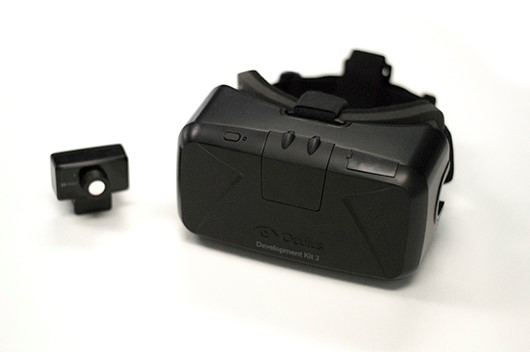
\includegraphics[width=0.45\textwidth]{dk2}
	\end{center}
	\vspace{-15pt}
	\captionsetup{width=0.42\textwidth}
	\caption{\textit{Oculus Rift DK2} mit externer IR-Kamera}\label{oculus}
	\vspace{-12pt}
\end{wrapfigure}
Bei dem \textit{Oculus Rift} handelt es sich um ein VR System. Den Entwicklern war es wichtig, dass sie mit dem \textit{Oculus} eine günstige VR-Lösung für jedermann anbieten können. Die erste Version des \textit{Oculus}, besitzt ein einfaches Display, den standartmässigen 3-DOF Sensor zur Orienterungsbestimmung und eine vollständige Integration in die Gameengin Unity, mit welcher Applikationen für die gängigen Betriebsysteme Windows, Mac und Linux, geschrieben werden können.\cite{website:oculus1}\\[6pt]
Da das Projekt mit Crowdfunding auf \textit{Kickstarter.com} finanziert wurde\cite{website:ocukick}, waren die Prototypen sehr schnell verbreitet und in kurzer Zeit wurden die ersten Abänderungen der Hardware für eine Video-See-Through-AR Erfahrung in den Foren diskutiert.\cite{website:arrift}\\[6pt]
Die nächste Version, unter dem Projektnamen ''Crystal Cove'' bekannt, verfügt über ein hochauflösendes Display und ein verbessertes Headtrackingsystem. Mithilfe einer IR-Kamera ist es nun möglich nicht nur die Lage der Brille sondern die genaue Position im Raum zu bestimmen. Es kann somit nicht von einem 6-DOF Sensor gesprochen werden. Kameras zur offiziellen AR Unterstützung sind jedoch immer noch nicht vorhanden und durch das neue Trackingsystem, welches eine externe Kamera benötigt, rückt die Vorstellung für eine mobile Anwendung in die Ferne.\cite{website:oculus2}
\newpage
\section{Weitere Ausgabegeräte für VR/AR}\label{s.otherdevices}
\subsection*{Akustische Ausgabegeräte}
Wie bereits in Kapitel \ref{c.wasist} beschrieben müssen bei einer möglichst immersiven VR/AR Erfahrung mehrere Sinne angesprochen werden. Zusätzlich zum visuellen Sinn ist es ebenfalls möglich Geräusche zu generieren. In VR Umgebungen lassen Umgebungsgeräusche den Anwender die Welt realer erscheinen. Das Fehlen auditiver Feedbacks, z.B. beim Fallenlassen einer Kiste in der virtuellen Welt, würde zu einem Bruch in der angeblichen Realität führen.\\[6pt]
Mithilfe von Mehrkanalsystemen kann ein räumlicher Effekt entstehen (wie man es aus Dolby Surround Sound kennt). Eine Weiterentwicklung dieses Systems ist die Wellenfeldsynthese. Dabei wird das Wellenfeld realer Ereignisse aufgenommen und kann anschliessend als synthetisches Wellenfeld über mehrere Lautsprecher ausgegeben werden. Es ist somit möglich verschiedene Schallquellen an beliebigen Positionen in einem begrenzten Gebiet zu erzeugen.\cite[S.~154]{doerner13}
\vspace{-10pt}
\subsection*{Haptische Ausgabegeräte}
Haptische Ausgabegeräte sprechen den Tastsinn des Anwenders an (z.B. die haptischen Schuhe in Kapitel \ref{s.shoes}). Somit kann der Nutzer die virtuelle Welt nichtnur sehen und hören, sondern auch fühlen. Mittels Vibrationen wird schon seit längerer Zeit in Videospielen der Rückstoss von Geweheren simuliert. Subwoofer können ausserdem verwendet werden, um den Boden vibrieren zu lassen.\\[6pt]
Für ein haptisches Feedback sind die geometrischen Modelle, welche zur optischen Darstellung verwendet werden, wegen des hohen Detailgrades nicht gut geeignet. Deshalb sollte zur Verkürzung der Rechenzeit ein betreffendes Haptikmodell mit in die virtuelle Umgebung aufgenommen werden. Dies ist ebenfalls nötig, da der Mensch viel mehr haptische als visuelle Eindrücke pro Sekunde aufnehmen kann.\cite[S.~154~f.]{doerner13}
\newpage
\section{Positional Tracking}\label{s.positional}
Damit Augmentierungen perspektivisch korrekt dargestellt werden, ist es essentiell die Position und Blickrichtung des Betrachters zu kennen. Bei den hier vorgestellten Methoden wurde darauf geachtet, dass sie einen relativ geringen Rechenaufwand besitzen und somit für mobile Anwendungen genutzt werden können.
\vspace{-10pt}
\subsection*{Marken-Tracking}
Das markenbasierte Verfahren des optischen Trackings verwendet zur Vermeidung der Fehleranfälligkeit bei schlechter Beleuchtung, sowie Verringerung der Berechnungskomplexität spezifizierte Marker. Diese Marker können passiv Licht reflektieren oder aktiv emittieren. Schwarzweissmarken haben sich in der Praxis bewährt, da sie leicht herzustellen sind und selbst von einfachen Kameras bei schlechten Lichtverhältnissen gut erkannt werden. Trotz ihrer Ähnlichkeit sollten sie nicht mit QR-Tags verwechselt werden. Während aus einem QR-Code die gesamte Information als Text entschlüsselt werden kann handelt es sich bei Markern lediglich um ein einfach zu erkennendes Muster, welches in einer Datenbank abgeglichen wird. Daraus folgt, dass es unmöglich ist die Augmentierung, welche an einen gegeben Marker gebunden ist, zu sehen. Dies ist nur möglich, sofern die vorhandenen Informationen aus einer Datenbank verfügbar sind. Diese Marken reichen vollkommen aus, falls das Tracking nur die Position des Objekts erkennen soll. Soll jedoch auch die Orientierung bestimmt werden müssen sogenannte Targets verwendet werden.\cite[S.~104~ff.]{doerner13}
\newpage
\begin{wrapfigure}{r}{0.35\textwidth}
	\vspace{-15pt}
	\begin{center}
		
\includegraphics[width=0.3\textwidth]{marken}
	\end{center}
	\vspace{-15pt}
	\captionsetup{width=0.3\textwidth}
	\caption{Beispiel-marken für Marken-Tracking}\label{marken}
	\vspace{-12pt}
\end{wrapfigure}
Die grösse der Marker ist entscheidend, da sie entweder nicht komplett erkannt werden können oder bei zu kleinen Marken die Anzahl der Markerpixel zu gering ist und es deshalb zu Fehlern in der Mustererkennung kommt. Durch einen zu flachen Betrachtungswinkel, können Transformationswerte stark schwanken und es kommt ebenfalls zu einer fehlerhaften Mustererkennung. Der grösste Nachteil solcher Marken ist der, dass sie direkt an dem zu augmentierenden Objekt angebracht werden müssen. Manchmal ist dies nicht möglich, sie würden vom Benutzer selbst verdeckt, wenn er das Objekt in die Hand nehmen müsste oder störend auffallen, da die Marker visuell nicht sehr ansprechend sind.\cite[S.~256~ff.]{doerner13}\\[6pt]
\vspace{-20pt}
\begin{wrapfigure}{l}{0.35\textwidth}
	\vspace{-30pt}
	\begin{center}
		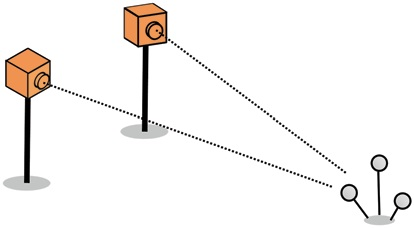
\includegraphics[width=0.3\textwidth]{target}
	\end{center}
	\vspace{-15pt}
	\captionsetup{width=0.3\textwidth}
	\caption{Tracking eines Targets mit mehreren Kameras}\label{target}
	\vspace{-12pt}
\end{wrapfigure}

Ein Target besteht aus mehreren Einzelmarken, von welchen die relative Position zueinander bekannt ist. Durch verschiedene Bauweisen von mehreren Targets kann das System diverse Objekte differenzieren. Wird mit solchen Targets gearbeitet, müssen mindestens zwei Kameras, je nach Grösse des zu überwachenden Gebiets auch mehr, benutzt werden. Die Bilddaten der einzelnen Kamera liefern bei einer Vorverarbeitung eine genaue Position in der zweidimensionalen Ebene. Mithilfe der zweiten Kamera ist es anschliessend möglich die genaue Position im Raum zu bestimmen.\cite[S.~106~ff.]{doerner13}
\newpage
\subsection*{Parallel Tracking and Mapping}
\begin{wrapfigure}{r}{0.35\textwidth}
	\vspace{-30pt}
	\begin{center}
		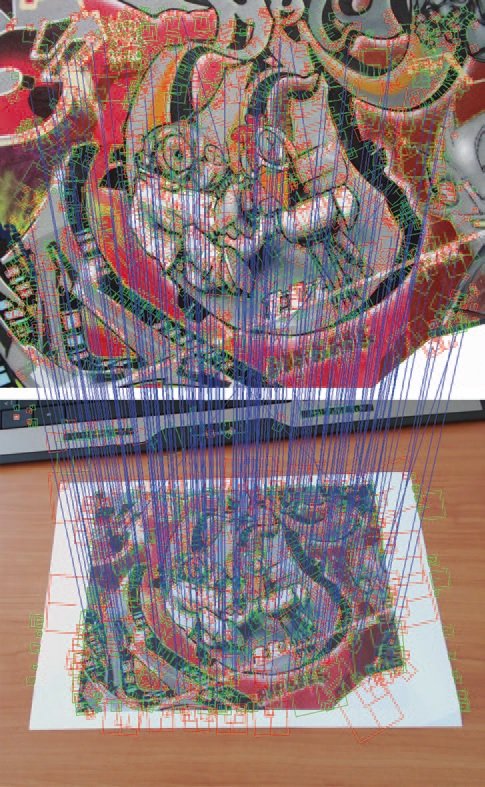
\includegraphics[width=0.3\textwidth]{features}
	\end{center}
	\vspace{-15pt}
	\captionsetup{width=0.28\textwidth}
	\caption{Zuordnung von Features des Kamerabildes zu einer Featuremap}\label{features}
	\vspace{-20pt}
\end{wrapfigure}
Wie im vorhergehenden Abschnitt bereits erwähnt, ist es nicht immer möglich Marken an zu augmentierende Objekte anzubringen. Eine Lösung zu diesem Problem bietet PTAM. Hierbei handelt es sich um ein markerloses Trackingverfahren. Es werden dazu Features (Kanten und Eckpunkte) aus dem Bild, welches in verschiedenen Auflösungen zur Verfügung steht, extrahiert und mit dem zuvor aufgenommenen Frame verglichen. Somit kann die Änderung des Blickwinkels berechnet werden.\cite[S.~106~ff.]{doerner13}\\[6pt]
PTAM verwendet im Gegensatz zu üblichen markerlosen Trackingverfahren eine geringere Anzahl von Features. Dies resultiert in einer geringeren CPU-Auslastung und verringert ausserdem Messfehler aufgrund von Bewegungsunschärfe, falls der Blickwinkel rasch verändert wird.\cite{website:ptam}

\subsection*{Differential Global Positioning System und Satellite Based Augmentation System}
Für Outdoor-AR-Anwendung bieten sich am ehesten DGPS und SBAS zur Positionsbestimmung an. Bei GPS können Abweichungen von 10 Metern oder mehr auftreten. Besonders in Wäldern oder Häuserschluchten kann die Position mit GPS nicht mehr genau bestimmt werden. Bei DGPS wird mithilfe eines lokalen Referenzempfängers ein Korrektursignal berechnet. Nachdem das Signal über Funkt oder Internet an den GPS-Empfänger gesendet und mit dessen Signal verrechnet wurde, ist eine Genauigkeit von bis zu wenigen Zentimetern möglich.\\[6pt]
\newpage
SBAS nutzt mehrere geostationäre Satelliten als Refernzsystem und ist deshalb nur in bestimmten Gebieten verfügbar (zurzeit Europa, Nordamerika und Japan). Dieses System verfügt über eine Abweichung von ca. einem Meter, kann jedoch bei eingeschränkter Sicht nach Süden fehleranfällig sein, da die Umlaufbahn geostationärer Satelliten über dem Äquator liegt. Bei der Augmentierung von Gebäuden und Gegenständen im Freien reicht die Genauigkeit jedoch aus, falls sich der Betrachter nicht allzu nah am Objekt befindet.\cite[S.~253~ff.]{doerner13}

\chapter{Virtual and Augmented Reality Town}\label{c.towndemo}
\vspace{-20pt}
\section{Motivation}\label{s.vrintro}
Ziel des Pilotprojekts war es herauszufinden, welche technischen Möglichkeiten es mit dem \textit{Oculus} und der dazugehörigen Engine \textit{Unity} gibt und welche Herausforderungen bei der Erstellung grosser virtueller Welten mit hohen Detail, in diesem Fall das St. Johann Gebiet mit einer Präzsision von 0.01 Meter Abweichung im 3D-Modell und einer grösse von 160 Hektare, auftreten. Neben dem Erstellen einer einfachen Simulation, sollte auch die Steigerung der Immersion einen grossen Stellenwert innerhalb des Projekts einnehmen. Dazu wurde ein VR Prototyp erstellt, welcher es dem Nutzer ermöglicht, sich im Stadtquartier St. Johann virtuell zu bewegen. Mithilfe des ''Flugmodus'' können Gebäude aus unterschiedlichsten Perspektiven betrachtet oder, dank der erhöhten Bewegungsgeschwindigkeit in der Luft, in kurzer Zeit grössere Distanzen zurückgelegt werden. Zur Steigerung der Immersion wurden ein möglichst realistischer Himmel und Umgebungsgeräusche, wie Verkehr in der Nähe von Strassen und Vogelgesang bei Bäumen, implementiert.\\[6pt]
Für die Implementierung konnte ein 3D Modell des Gebietes, welches von der Stadt Basel zur Verfügung gestellt wurde, verwendet werden. Mithilfe der \textit{Unity} Engine, welche ein offizielles SDK für den \textit{Oculus Rift} besitzt, konnte ein VR Prototyp realisiert werden. Neben der erwähnten Engine wurde \textit{Google Sketchup} zur Anpassung des Stadtmodells und eine in \textit{Eclipse} geschrieben Java-Applikation zur Erstellung der Bodentextur verwendet.
\newpage
\section{Kalibrieren des virtuellen Terrains}\label{s.terrain}
Mithilfe von \textit{Google SketchUp} ist es möglich 3D-Modelle von Gebäuden zu kreieren oder bereits vorhandene Modelle zu importieren und ihre Grösse zu ändern. Da das Stadtmodell bereits vorhanden war, mussten keine Gebäude erstellt werden und nach dem Import kann mithilfe der Geostandort Funktion in \textit{SketchUp} ein Satellitenbild von Google importiert werden. Damit können die Gebäude korrekt kalibriert werden und liegen somit in \textit{Unity} in der richtigen Grösse vor.

\begin{figure}[htp]%
	\centering	
	\subfigure[][]{%
		\label{fig:preska}%
		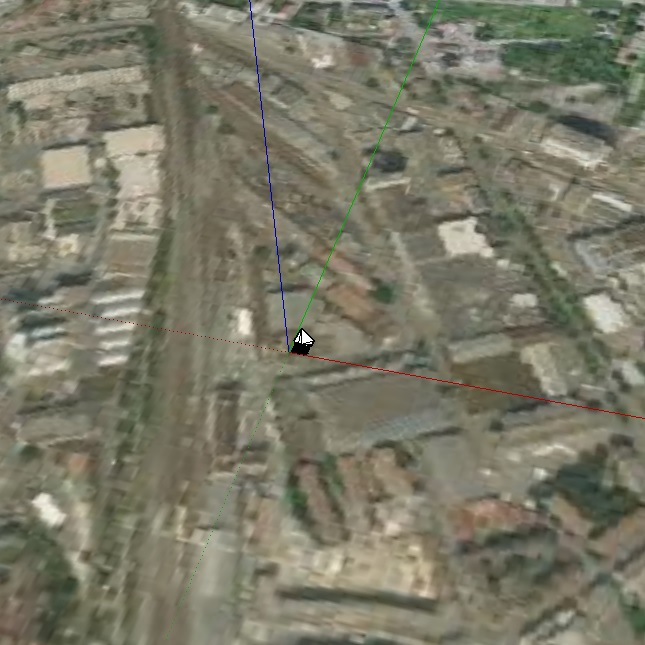
\includegraphics[width=0.4\textwidth]{preska}}%
	\hspace{48pt}%
	\subfigure[][]{%
		\label{fig:anteska}%
		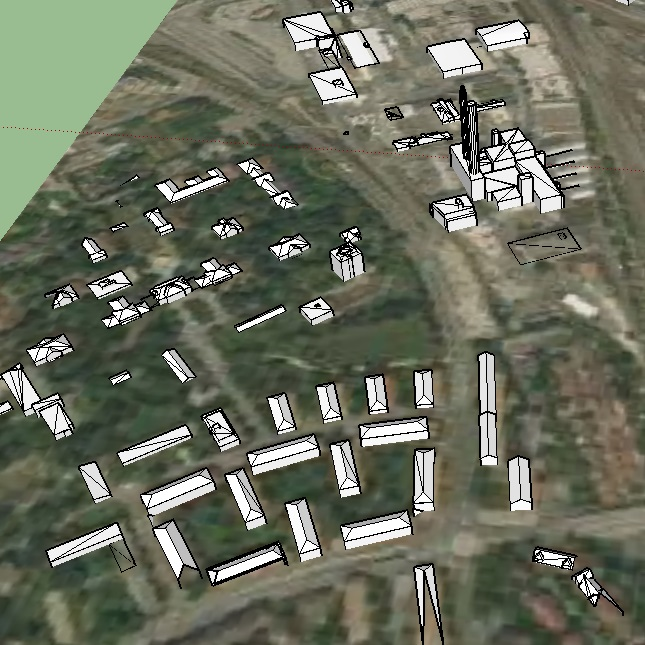
\includegraphics[width=0.4\textwidth]{anteska}}%
	\hspace{8pt}%

	\caption[3D-Modell mit \textit{SketchUp} skalieren]
	{3D-Modell mit \textit{SketchUp} skalieren:
		\subref{fig:preska} Stadtmodell mit Geostandort vor und
		\subref{fig:anteska} nach der Skalierung in \textit{SketchUp}}%		
	\label{fig:sketchup} %
\end{figure}

In Abbildung \ref{fig:preska} ist das Stadtmodell als kleine weisse Fläche im Zentrum des Bildes zu erkennen.  Mit dem Skalierungstool in \textit{SketchUp} kann das gesamte Modell so weit vergrössert werden, bis Position und Grösse der Gebäude mit ihren realen Gegenstücken auf dem Satellitenbild übereinstimmen. Dies ist für das weitere Vorgehen wichtig, damit in \textit{Unity} das Verhältnis zwischen den Grössen des Beobachterobjekts (Augenhöhe, Schrittweite) und des Modells übereinstimmt.\\[6pt]
Anschliessend wird das so korrigierte Modell als eine für \textit{Unity} kompatible OBJ-Datei exportiert. Bei einer OBJ-Datei handelt es sich um ein simples Format zum Speichern von 3D-Modellen. Es besteht aus mehreren Listen, mit welchen die einzelnen Flächen des Modells beschrieben werden. Zum einen ist eine Sammlung von Eckpunkten und Normalen vorhanden und, falls zuvor definiert, sind Textur-Koordinaten ebenfalls angegeben. Des weiteren ist es möglich innerhalb der Datei die Flächen zu gruppieren. Da die Unterscheidung der verschiedenen Flächen in ''Wände'',''Dächer'' und ''Terrain'' innerhalb der zugrunde liegenden DXF-Datei vorhanden ist, bleibt beim Export diese Information erhalten und kann später in \textit{Unity} verwendet werden um unterschiedliche Texturierungen an diesen Oberflächen automatisch anzubringen. So können Dächer rot und Wände grau eingefärbt werden, siehe Abbildung \ref{unity}.\\[6pt]

\begin{figure}[hbt]
	\vspace{-25pt}
	\begin{center}
		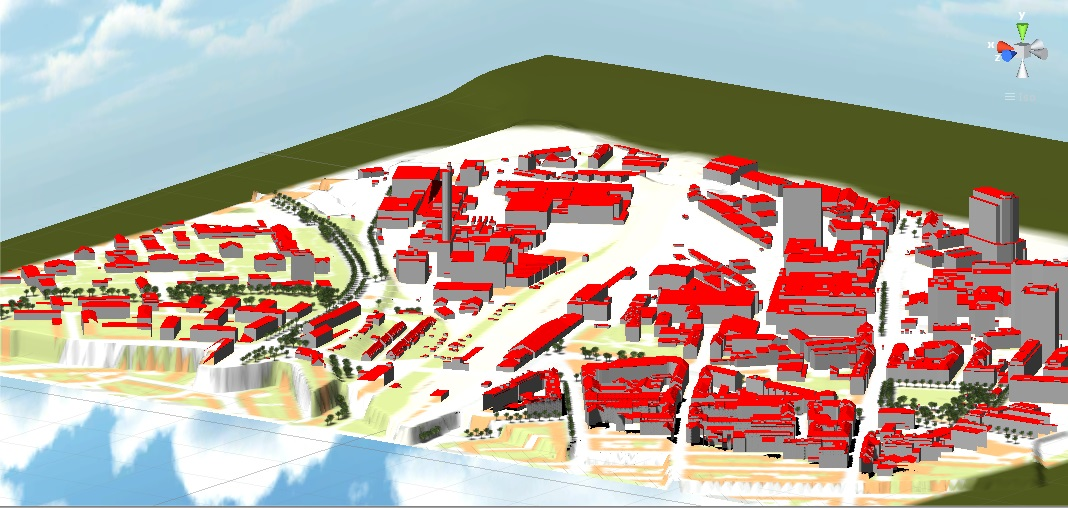
\includegraphics[width=1\textwidth]{unity}
	\end{center}
	\vspace{-15pt}
	\caption{VR St. Johann in Unity}\label{unity}
	\vspace{-15pt}
\end{figure}

Damit auf terraineigene Funktionen wie das Hinzufügen von Pflanzen und Bäumen sowie die Verwendung einer Karte als Textur zugegriffen werden kann, muss die Fläche, welche das Terrain beschreibt, mithilfe des Skripts \textit{Object2Terrain}\cite{website:terrain} in ein spezielles \textit{Terrainobjekt} umgewandelt werden.\\[6pt]
Für die Terraintextur kann eine hochauflössende Karte des Gebiets verwendet werden. Diese kann mit einer innerhalb dieser Arbeit erstellten Java-Applikation automatisch zusammengestellt werden. Die Anwendung lädt kleinere Kartenausschnitte im Massstab 1:500 mit hoher Auflösung aus dem \textit{Geoviewer} der Stadt Basel und kombiniert diese zu einer grossen zusammenhängenden Karte. Bei den kleineren Kartenausschnitten handelt es sich um Quadrate (sogenannte Tiles) mit einer Abmessung von 256 Pixel Kantenlänge. Sie stellen ein Gebiet von ca. 12 Are dar. Das Resultat ist eine quadratische Karte mit einer Kantenlänge von 9216 Pixeln und ein Gebiet von etwa 160 Hektare umfasst. Der Sourcecode sowie die erstellte Karte befindet sich im Anhang unter \ref{s.tilegrabber}.\\[6pt]
Die Immersion kann mit dem Einfügen weiterer Objekte gesteigert werden. Da auf der Karte Details wie die Position einzelner Bäume vermerkt sind, können mit dem in \textit{Unity} integrierten Tool unterschiedliche Bäume manuell positioniert werden. Zudem ist es möglich Verkehrsgeräusche in der Nähe von Strassen einzufügen. In \textit{Unity} stehen dazu eigene Tonquellenobjekte zur Verfügung, welche die Lautstärke bei der Entfernung des Nutzers von der Tonquelle möglichst realistisch reduzieren.\\[6pt]
\vspace{-12pt}
\begin{wrapfigure}{r}{0.35\textwidth}
	\vspace{-30pt}
	\begin{center}
		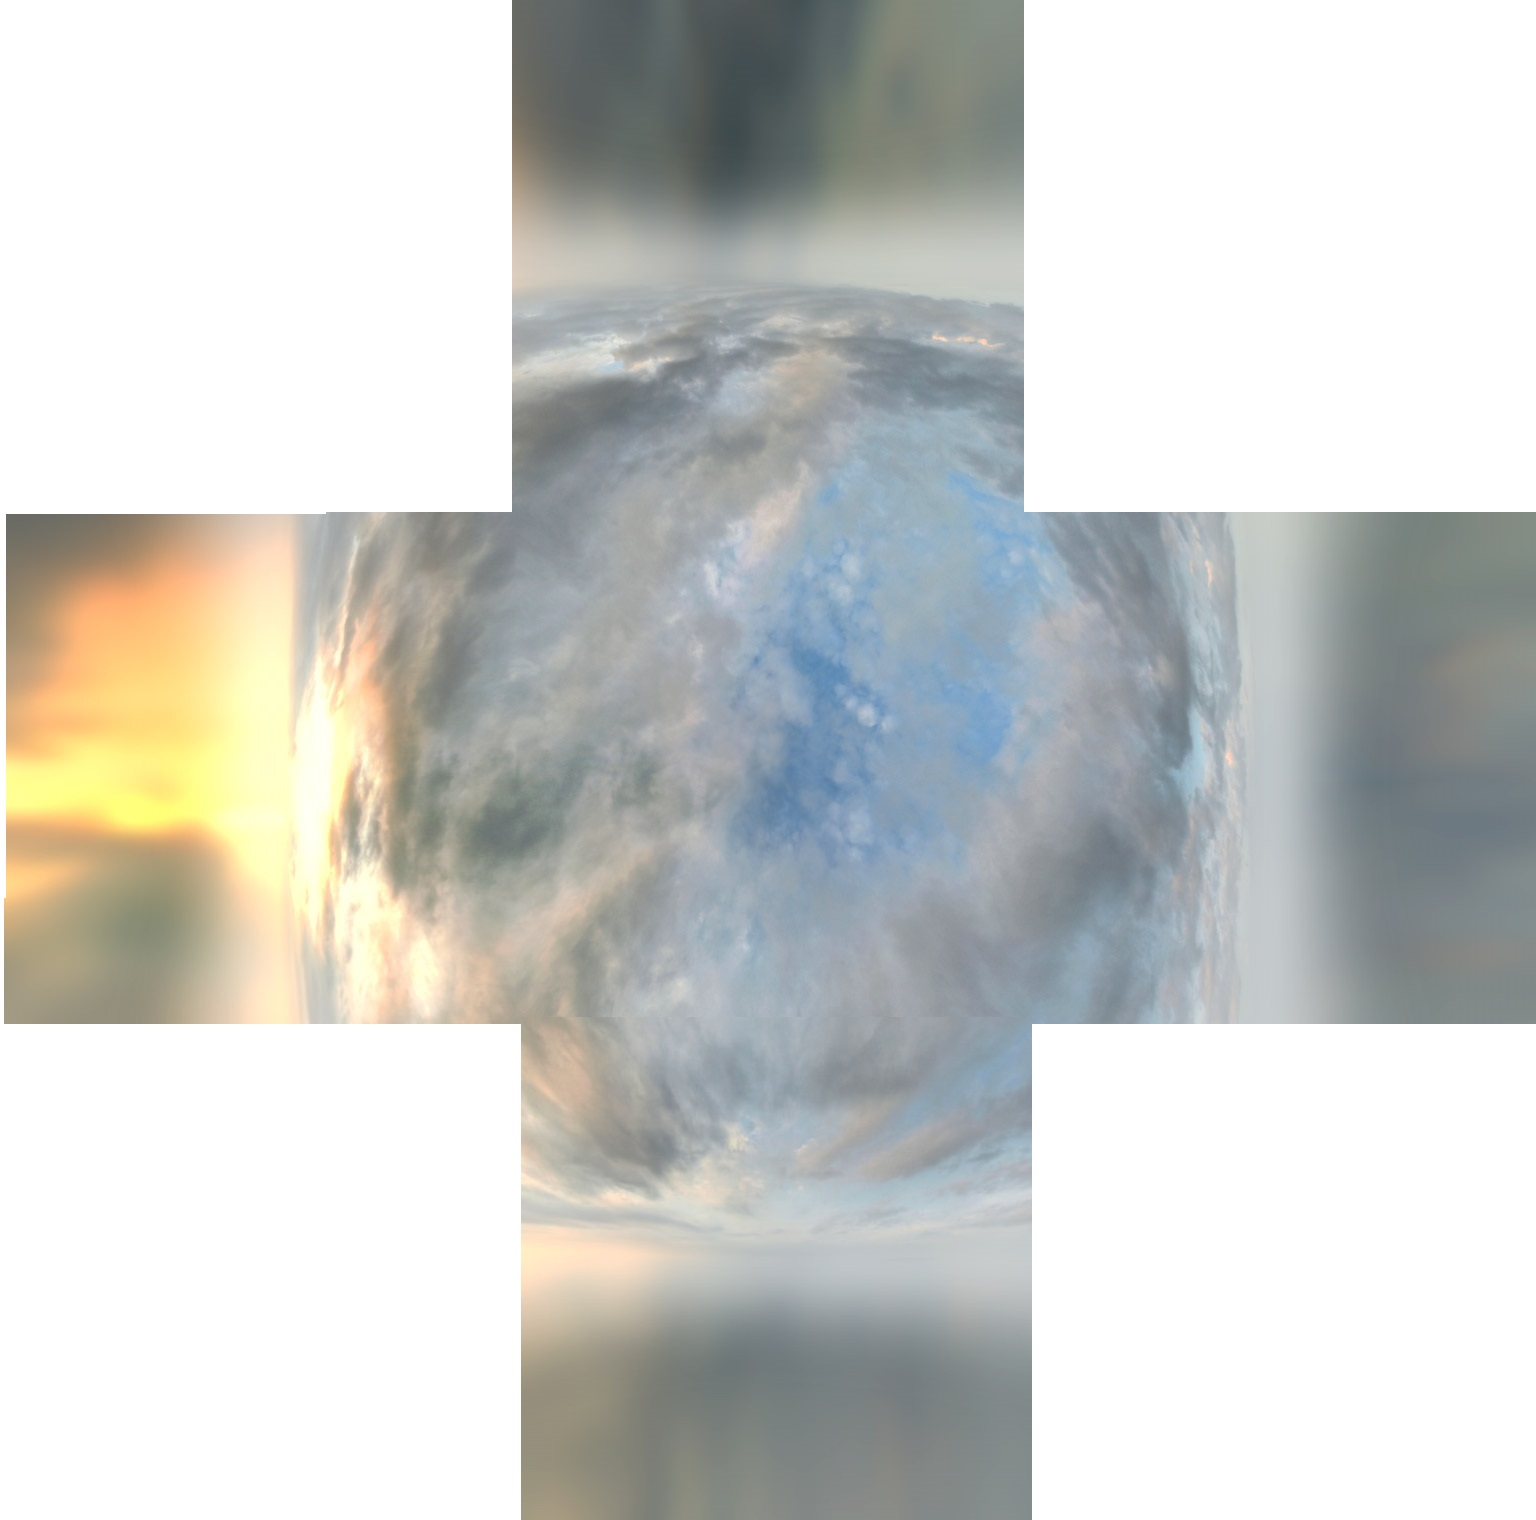
\includegraphics[width=0.3\textwidth]{Skybox}
	\end{center}
	\vspace{-15pt}
	\captionsetup{width=0.28\textwidth}
	\caption{Die Texturen einer Skybox}
	\vspace{-20pt}
\end{wrapfigure}
Um einen realistischen Himmel darzustellen kann eine Skybox verwendet werden. Hierbei handelt es sich um einen Würfel ohne Boden, welcher die Welt umschliesst und inwändige Texturen besitzt. In \textit{Unity} sind diverse Textursets bereits vorhanden, welche unterschiedliche Wettersituationen darstellen. Nach dem die Skybox integriert wurde, kann eine Lichtquelle, welche die Sonne der virtuellen Welt darstellen wird, an die Position der Sonne in der Textur gezogen werden. Da es sich hier ebenfalls um ein \textit{Unity} eigenes Objekt handelt können spezielle Einstellungen wie Blendeffekte eingefügt werden. Wendet der Nutzer nun seinen Blick in die Richtung der Sonne auf der Skybox, wird er von ihr bzw. der Lichtquelle, welche sich an der selben Position befindet, geblendet. Würde dieser Effekt nicht auftreten, käme es zu einem Bruch der Realität und die Anwendung würde einen relativ hohen Grad an Immersion einbüssen. Ausserdem ist es nun möglich eine Shadowmap mithilfe eines Assistenten in wenigen Schritten zu kreieren und somit den wirklichen Schattenwurf der Gebäude darzustellen. Grundsätzlich erstellt \textit{Unity} ein Bild der virtuellen Welt aus Sicht der Lichtquelle. Alle Objekte, welche von der Lichtquelle aus gesehen verdeckt sind, liegen im Schatten.\\[6pt]


\section{Hinzufügen des Beobachterobjekts}\label{s.ovr}
Mithilfe des zur Verfügung gestellten SDK von \textit{Oculus} kann ein für den HMD konzipiertes Beobachterobjekt in die Welt eingefügt werden. Es verfügt bereits über grundlegende Bewegungen wie Springen, Laufen oder Rennen und verwendet die Informationen des integrierten 3-DOF Sensors um die Bewegungen des Kopfes in der Realität ebenfalls in der virtuellen Welt umzusetzen.\\[6pt]

\begin{figure}[htb]
	\vspace{-20pt}
	\begin{center}
		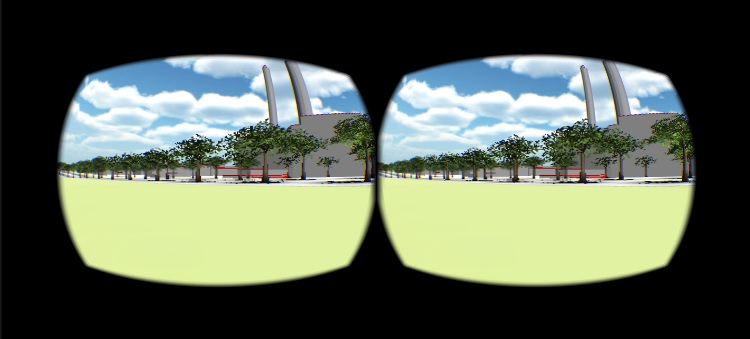
\includegraphics[width=0.8\textwidth]{oculusvision}
	\end{center}
	\vspace{-15pt}
	\caption{Sicht des Beobachterobjekts}\label{oculusvision}
	\vspace{-12pt}
\end{figure}

 Ausserdem werden die Inhalte bereits korrekt als das für den \textit{Oculus} charakteristische Doppelbild ausgegeben, auch \textit{Oculus Vision} genannt. Dieses ist in Abbildung \ref{oculusvision} zu sehen. Da mit speziellen Linsen im \textit{Oculus} das Bild über das gesamte Sichtfeld dargestellt werden kann müssen nicht alle Pixel berechnet werden und der nicht sichtbare Bereich kann, um Rechenaufwand einzusparen, als einfache schwarze Fläche dargestellt werden.\\[6pt]
Um dem Benutzer die Möglichkeit zu geben, sich schnell von Punkt A nach B zu bewegen und einen besseren Überblick über die Szene zu haben, kann ein ''Flugmodus'' implementiert werden\footnote{siehe \ref{s.flug}}. Dazu werden die Funktionen, welche für den Sprungbefehl verantwortlich sind, in der Klasse des Beobachterobjekts abgeändert. Solange die Taste für den Sprung gedrückt wird, wirkt keine Gravitation auf den Nutzer und er schwebt in der Luft. Wird die Taste losgelassen sinkt er wieder zu Boden. Es ist ausserdem möglich die Bewegungsgeschwindigkeit stark zu erhöhen, falls sich der Nutzer nicht auf dem Boden befindet.

\section{AR Town}\label{c.artown}
Hier werden die theoretischen Überlegungen, wie man die erstellte VR Anwendung in eine AR Applikation weiterentwickeln kann, ausgeführt. Um dies zu bewerkstelligen müssen einerseits Änderungen an der Hardware, sprich anbringen einer Stereokamera und gegeben falls Sensoren f"ur die Positionsbestimmung, und andererseits der Programmcode umgeschrieben werden.\\[6pt]
Da es sich beim \textit{Oculus Rift} um einen geschlossenen HMD handelt, müssen Videokameras angebracht werden um aus dem VR System ein Video See-Through-AR System zu erstellen. Bei den Kameras ist darauf zu achten, dass sie mindestens 60 Bilder pro Sekunde aufnehmen, um ein flüssiges Bild garantieren zu können. Ausserdem ist ein möglichst grosser Aufnahmewinkel nötig, da der Oculus selbst über ein relativ breites Sichtfeld verfügt und ansonsten schwarze Ränder entstehen würden.\cite{website:arrift}\\[6pt]
Zur Positionsbestimmung kommen mehrere Alternativen in Frage (siehe \ref{s.positional}). Da die Applikation mehrheitlich im Freien genutzt wird, bietet sich am ehesten DGPS an. Eine andere Möglichkeit wäre eine Kombination aus dem vorgestellten PTAM, dem Multiple Maps System der selben Arbeitsgruppe\cite{website:multimaps} und GPS. Mithilfe von GPS wird die Position grob bestimmt und anschliessend mithilfe des Multiple Maps System die verschiedenen Featuremaps der Umgebung geladen. Anschliessend kann mithilfe von PTAM die Augmentierung richtig positioniert werden.\\[6pt]
\newpage
Im Programmcode müssen dementsprechend Änderung angebracht werden. So muss das gewonnen Doppelbild als steter Hintergrund der Szene verwendet werden. Möchte man dass Bäume, Baugerüste oder andere Gebäude das virtuelle Objekt verdecken können, muss eine Methode gefunden werden, welche die vorhandenen realen Objekte erkennt und das 3D-Modell an den entsprechenden Stellen zuschneidet.

\chapter{Einblicke in Programmiertechniken}\label{c.programing}
\vspace{-20pt}
\section{Einführung in Unity}\label{s.unity}
Mit dem erwerb des \textit{Oculus Rift} erhält man eine drei monatige Lizenz für \textit{Unity}, welche verwendet werden kann um VR-Simulationen zu kreieren. Die freie Lizenz, unter welcher \textit{Unity} ebenfalls erhältlich ist, ist für die Programmierung mit dem \textit{Oculus} nicht geeignet, da sie die zuvor erwähnte \textit{Oculus Vision} nicht unterstützt.\\[6pt]
Bei \textit{Unity} handelt es sich um eine Engine, welche zur Computerspielentwicklung genutzt wird. Sie verfügt bereits über grundlegende Objekte, welche für die Erstellung einer virtuellen Welt nötig sind. Eine übersichtliche Oberfläche und ''Drag and Drop'' Funktion ermöglicht eine schnelle Arbeitsweise und leichte Bedienung. Möchte man Anpassungen an bereits bestehenden Funktionen (wie z.B. der oben beschriebene ''Flugmodus'', welcher durch das Anpassen der Sprungfunktion realisiert wurde) können die einzelnen Funktionen, welche in \textit{Unity} Skripte genannt werden, verändert oder neu implementiert werden. Als Programmiersprache akzeptiert die Engine JavaScript oder C\#. Es ist auch möglich durch den integrierten Store Skripte und Assets (Sammlung von Skripten, 3D-Modellen, usw.) von anderen Programmierern zu erwerben und in sein Programm einzubinden. Diese reichen von einfachen kostenlosen Skripten wie dem \textit{Object2Terrain}, welches in Kapitel \ref{s.terrain} erwähnt wurde bis zu grossen Sammlungen von 3D-Modellen von z.B. Bäumen, Fahrzeugen, Häuser oder anderen Objekten.\\[6pt]

\newpage
\begin{figure}[ht]
	\vspace{-20pt}
	\begin{center}
		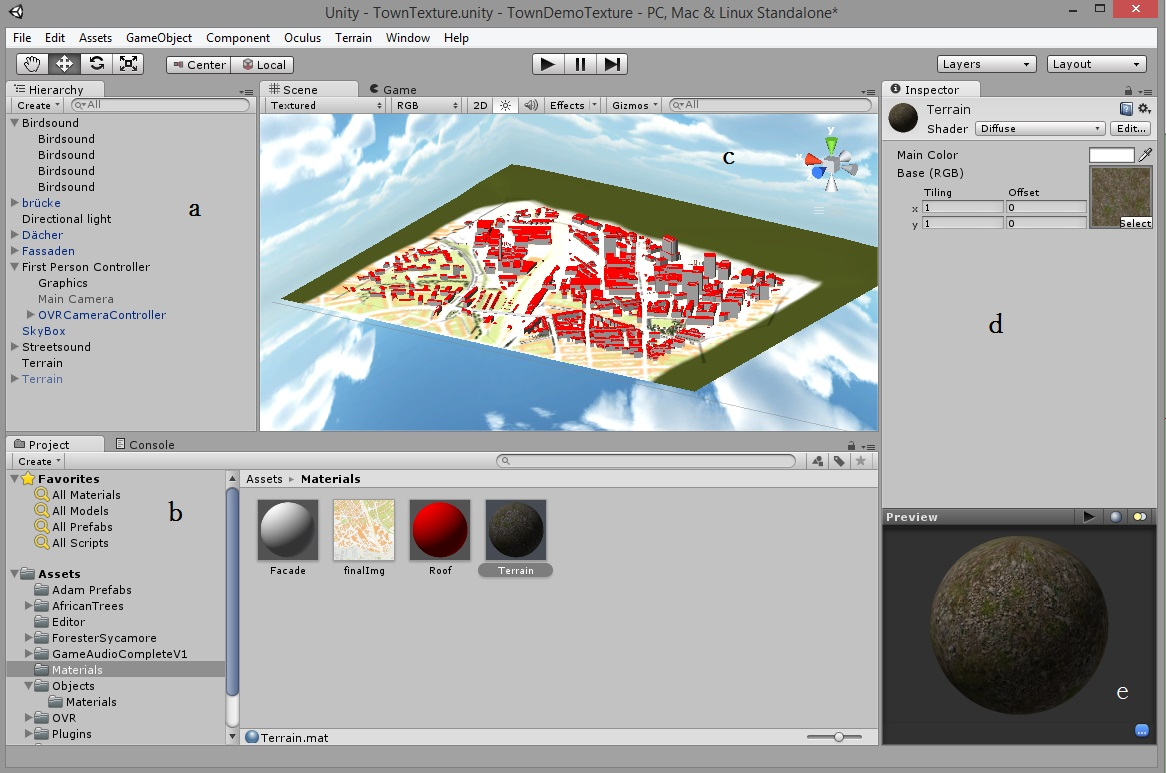
\includegraphics[width=1\textwidth]{unityall}
	\end{center}
	\vspace{-15pt}
	\caption[Maske der Unity Engin]{Maske der Unity Engin: (a) Objektexplorer, (b) Dateiexplorer, (c) Scene Preview, (d) Inspector, (e) Object Preview}\label{unityall}
	\vspace{-12pt}
\end{figure}

 In Abbildung \ref{unityall} wird die Maske von \textit{Unity} gezeigt. Alle Elemente, welche in (a) enthalten sind, sind in die Welt integriert. Erscheint der Name des Objekts grau, ist es deaktiviert (in diesem Fall die Hauptkamera, da der Oculus Rift verwendet wird und somit die OVRCameraController aktiviert sein müssen). Hier ist es auch möglich einzelne Elemente zu einer Gruppe zusammenzufassen. Neben einer besseren Übersicht bietet dies die Möglichkeit Vater-Kind-Beziehungen herzustellen. Bewegt sich nun der ''First Person Controller'' so wird auch der ''OVRCameraController'' in die selbe Richtung bewegt. In (b) sind hingegen die Dateien, welche bereits in \textit{Unity} importiert jedoch noch nicht unbedingt verwendet wurden, angezeigt. Dies sind die sogenannten ''Assets''. Durch klicken der rechten Maustaste in diesem Feld können weitere Elemente importiert werden. Mithilfe einer ''Drag and Drop'' Funktion können Elemente von (b) sowohl in (a) oder gleich in das Vorschaufenster (c) an die richtige Position gezogen werden. In (d) sind weitere Informationen zum ausgewählten Objekt zu finden. Bei Spielerobjekten wäre dies z.B. die Höhe der Figur, seine Laufgeschwindigkeit, die Sprunghöhe und im Falle des \textit{Oculus} auch sein Augenabstand. Das letzte Feld (e) ist lediglich eine Vorschau des ausgewählten Objekts, unter der Voraussetzung, dass es sich dabei um eine Textur oder ein 3D-Modell handelt.\\[6pt]
 Ist das Programm fertiggestellt und bereit kompiliert zu werden, kann über einen Assistenten das Zielsystem gewählt werden und \textit{Unity} gibt anschliessend eine ausführbare Datei aus. Die Anwendung kann neben Windows, Linux und Mac auch für mobile Plattformen wie Android, iOS, Windows Phone und Blackberry 10 oder gar als Webplugin zur Integration in eine Webseite kompiliert werden. Abbildung \ref{UnityArchitektur} zeigt einen Überblick, wie die einzelnen Teile zusammenarbeiten.\\[6pt]
 \newpage
 

 \begin{figure}[ht]
 	\vspace{-15pt}
 	\begin{center}
 		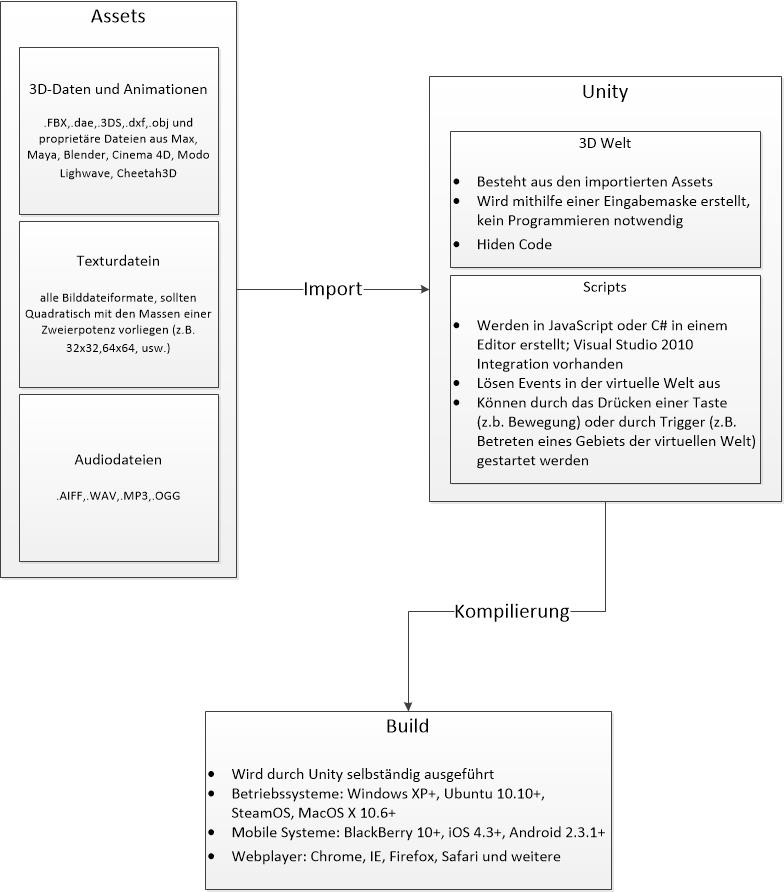
\includegraphics[width=0.9\textwidth]{UnityArchitektur}
 	\end{center}
 	\vspace{-15pt}
 	\caption[Unity Architektur]{Übersicht von Unity}\label{UnityArchitektur}
 	\vspace{-12pt}
 \end{figure} 
 
 
 
 
 
\newpage
\section{Use-Case: Hinzufügen einer Brücke}\label{s.brücke}
In dem zur Verfügung gestellten 3D-Modell des St. Johann Quartiers hat die Brücke über die Bahngleise in der Nähe des Lothringerplatzes gefehlt. Durch das Hinzufügen des Geostandorts konnten die Informationen von \textit{Google Maps} genutzt werden um den Verlauf der Brücke realitätsnah nachzubilden. Mithilfe des Zeichentools kann eine Fläche, welche der Form der Brücke entspricht, gezeichnet werden. Anschliessend kann diese Fläche in der Höhe gestreckt und somit zu einem dreidimensionalen Körper transformiert werden. Nach dem Export besitzt die Brücke bereits über die richtige Grösse, da das restliche Stadtmodell wie oben erwähnt auch mit dem Geostandort skaliert wurde. Weitere Anpassungen sind nach dem Import in \textit{Unity} nicht mehr nötig.\\[6pt]

\begin{figure}[ht]
	\vspace{-20pt}
	\begin{center}
		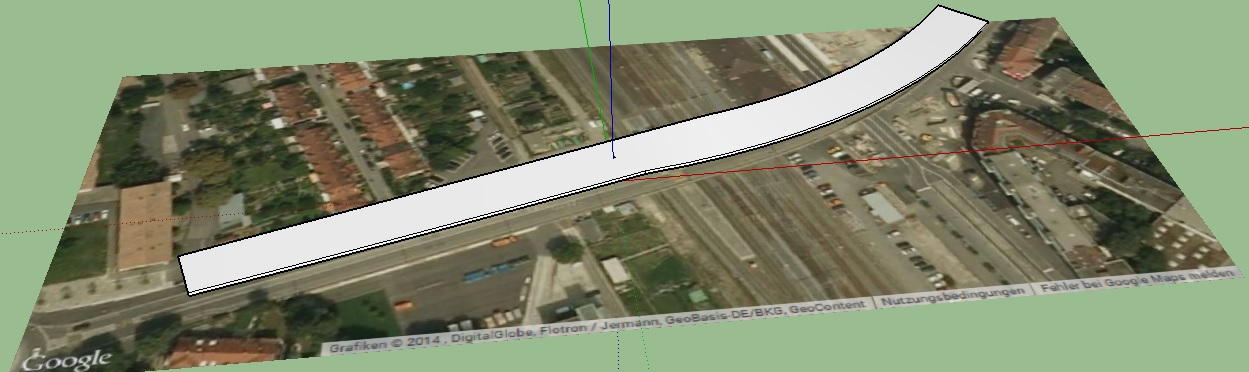
\includegraphics[width=0.8\textwidth]{sketchup}
	\end{center}
	\vspace{-15pt}
	\caption{Modell der Brücke in SketchUp}\label{sketchup}
	\vspace{-12pt}
\end{figure}

\newpage
In \textit{Unity} können sämtliche benötigte Dateien als ''Asset'' importiert werden. Grundlegend unterscheidet man drei Typen von Assets. Animationen und 3D-Modelle, Texturen und Tondateien. Bei den 3D-Formaten utnerstützt \textit{Unity} unter anderem FBX, Collada DAE und OBJ Dateien wie auch Dateiformate, welche von 3D Programmen wie Blender oder Maya erstellt wurden. Nach dem Import in Unity können die Assets aus dem Dateiexplorer in das Scene Preview Fenster an die korrekte Position gezogen werden. Anschliessend können im Inspector noch Änderungen am Objekt vorgenommen werden, in diesem Fall musste die Brücke um 2° auf der Y-Achse gedreht werden, damit sie mit dem Strassenverlauf übereinstimmt. Zudem wurde ein "Mesh Collider" hinzugefügt, damit der Anwender nicht durch die Brücke hindurch fällt, falls er versucht sie zu überqueren.\\[6pt]
 
 \begin{figure}[ht]
 	\vspace{-20pt}
 	\begin{center}
 		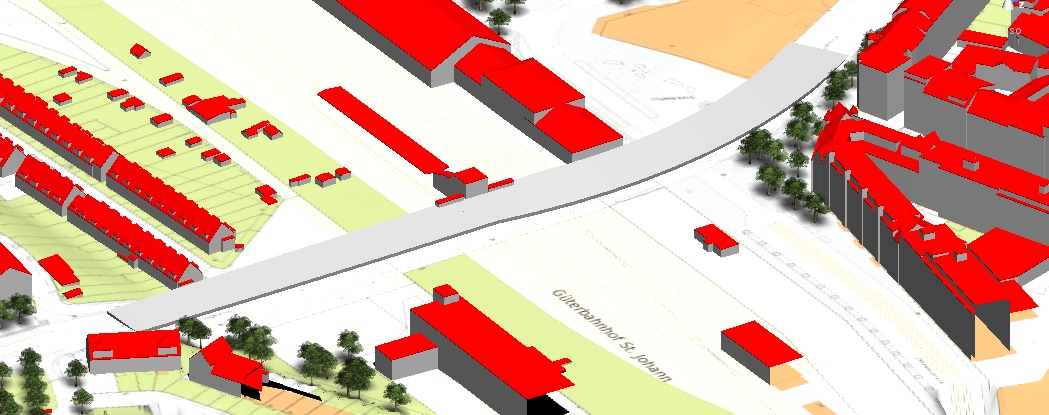
\includegraphics[width=0.8\textwidth]{unitybrucke}
 	\end{center}
 	\vspace{-15pt}
 	\caption{Modell der Brücke im VR St. Johann}\label{unitybrücke}
 	\vspace{-12pt}
 \end{figure}

\chapter{Schlusswort}\label{c.zusammenfassung}
\vspace{-20pt}
Das Schreiben dieser Arbeit weckte in mir den Pioniergeist. Beinahe wöchentlich wurden Informationen zu neuer Hardware oder VR/AR Projekten veröffentlicht. Die Begeisterung, welche AR momentan erfährt treibt die Entwicklung immer weiter voran und selbst der in diesem Projekt verwendete \textit{Oculus Rift}, welcher zu Beginn relativ neu war, kann bereits als veraltete Technologie bezeichnet werden. Doch selbst Systeme wie die erst kürzlich erschienene \textit{castAR} werden in wenigen Jahren belächelt.\\[6pt] 
Diese Arbeit soll ein erster Schritt in die Welt der VR/AR sein und einen groben Überblick in das Themengebiet geben. Das im Rahmen der Arbeit entwickelte Softwareprojekt läuft ohne Abstürze und dank \textit{Unity} konnte eine sehr grosse virtuelle Welt erstellt werden, welche auch auf Systemen mit geringerer Leistung flüssig läuft. Bei der Veränderung der Benutzerschnittstelle, wie bei der Implementierung des ''Flugmodus'', sind Programmierkentnisse im Bereich von JavaScript von nöten um den vorhanden Code zu verstehen und an den richtigen Stellen abzuändern. Der wohl schwierigste Teil war die Erstellung der hochauflösenden Karte. Ich wollte ein System entwickeln, welches später ermöglicht, mit wenigen Änderungen, eine Karte eines anderen Stadtquartiers zu erstellen. Da diese Karten jeweils nur als kleiner Ausschnitt auf dem Geoportal der Stadt Basel betrachtet werden konnten, mussten die einzelnen Teilkarten mit einem selbstentwickelten Programm zusammengeführt werden. In einer ersten Version war eine GUI geplant, über die der Kartenausschnitt auf einer Karte der ganzen Stadt Basel gewählt werden konnte und anschliessend eine detailierte Karte zusammengestellt wurde. Da aber keine Relation zwischen ''echten'' Koordinaten (z.B. LV95) und der internen Ablagestruktur gefunden wurde, war dies leider nicht möglich.\\[6pt]
 In Zukunft sollen dem Pilotprojekt weitere Funktionen hinzugefügt werden. So soll es irgendwann möglich sein ein zuvor bestimmtes Gebäude in der Höhe zu verändern und so seinen Einfluss auf das Stadtbild zu beobachten. Ausserdem sollen die wichtigsten Standorte bereits beim Programmstart als Einstiegspunkt genutzt werden können, damit ein Positionswechsel innerhalb der Anwendung nicht nötig wird und eine vereinfachte Steuerung, welche aus lediglich einer Taste zur Aktivierung des ''Flugmodus'' besteht, möglich wird.
% Anhang
%\begin{landscape}\begin{multicols}{2}
%\appendix
\chapter{Anhang}\label{c.anhang}
\vspace{-20pt}
\section{TileGrabber}\label{s.tilegrabber}
Mithilfe des TileGrabber Programms können Karten aus der Region Basel im Massstab 1:500 zusammengestellt werden. Da es keine Relation zwischen der Indexierung der einzelnen Teilbilder und geographischer Koordinaten (z.B. LV95) gibt, müssen Start und Endpunkt aus dem HTML Code ausgelesen werden. Das Programm sammelt anschliessend die Teilbilder von West nach Ost und von Nord nach Süd um sie schlussendlich in einem grossen Bild zusammenzufügen. Dieses kann anschliessend als Textur des Terrains benutzt werden.

\renewcommand{\baselinestretch}{1}\normalsize
\lstinputlisting[language=Java]{code/Main.java}
\renewcommand{\baselinestretch}{1.5}\normalsize
\begin{figure}[htp]%
	\centering
	\subfigure[][]{%
		\label{fig:map}%
		\includegraphics[width=0.9\textwidth]{map}}%
	\hspace{8pt}%
	
	\subfigure[][]{%
		\label{fig:mapdetail}%
		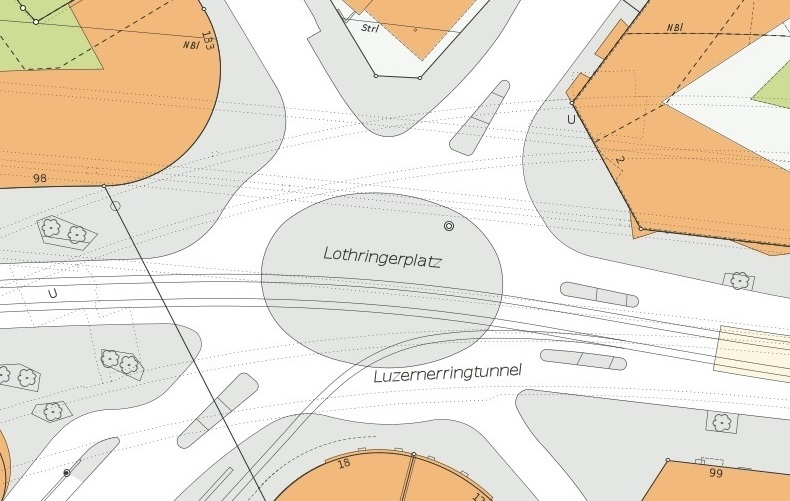
\includegraphics[width=0.4\textwidth]{mapdetail}}%
	\hspace{48pt}%
	\subfigure[][]{%
		\label{fig:vrdetail}%
		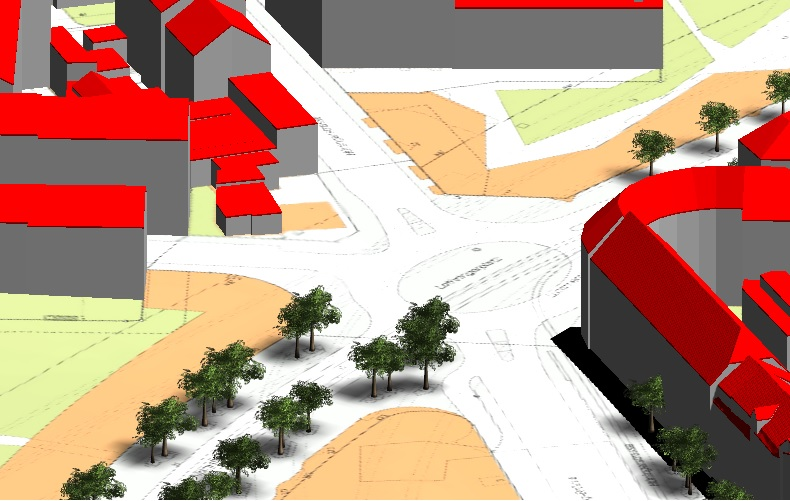
\includegraphics[width=0.4\textwidth]{vrdetail}}%
	\hspace{8pt}%

	\caption[TileGrabber Beispiele.]
	{TileGrabber Beispiele:
		\subref{fig:map} Gesamte Karte aus TileGrabber (Lothringerplatz markiert),
		\subref{fig:mapdetail} Detailansicht auf Lothringerplatz,
		\subref{fig:vrdetail} Lothringerplatz in VR.}%
\end{figure}


\newpage
\section{Flugmodus}\label{s.flug}
Aus Platzgründen werden hier nur Teile des Codes aufgeführt, welche für den ''Flugmodus'' abgeändert wurden. Alle Funktionen sind Bestandteil des Standartsskripts zur Charaktersteuerung in Unity. 
Um nach dem Springen in der Luft zu bleiben wurde in der Funktion \textit{ApplyGravityAndJumping} ein Else hinzugefügt, welches, solange die Springentaste gedrückt und die maximale Höhe noch nicht erreicht wurde, die Bewegung in y-Richtung ausser Kraft setzt. 

\renewcommand{\baselinestretch}{1}\normalsize
\lstinputlisting[language=c]{code/jumping.cs}
\renewcommand{\baselinestretch}{1.5}\normalsize

\newpage
Für die erhöhte Bewegungsgeschwindigkeit in der Luft wurde in \textit{GetDesiredHorizontalVelocity} ein Else hinzugefügt, welches die maximale Geschwindigkeit mit einem Wert multipliziert, solange man in der Luft ist.

\renewcommand{\baselinestretch}{1}\normalsize
\lstinputlisting[language=c]{code/fly.cs}
\renewcommand{\baselinestretch}{1.5}\normalsize

%\end{multicols}\end{landscape}

\bibliographystyle{alpha}
\bibliography{bibliographie}

\chapter*{Erklärung}
\vspace{-20pt}
Hiermit versichere ich, dass ich die vorliegende Arbeit selbstständig verfasst und keine anderen als die angegebenen Quellen und Hilfsmittel benutzt habe, dass alle Stellen der Arbeit, die wörtlich oder sinngemäß aus anderen Quellen übernommen wurden, als solche kenntlich gemacht und dass die Arbeit in gleicher oder ähnlicher Form noch keiner Prüfungsbehörde vorgelegt wurde.

\vspace{3cm}
Ort, Datum \hspace{5cm} Unterschrift\\

\end{document}